\chapter{CMB instrument overview}
\label{ch:cmb_instrument_overview}

One of the most powerful and prominent methods to study the Big Bang model laid out in Chapter~\ref{ch:scientific_motivation} is to study CMB temperature and polarization anisotropies with high precision. Such an endeavor requires specialized telescopes that are designed specifically to be sensitive at millimeter wavelengths. These telescopes are then used to map the CMB---or to measure its intensity and polarization fluctuations as a function of sky coordinate---by scanning its field of view across the sky.

Modern-day CMB instruments are \important{background limited}, meaning that their sensitivity is limited by fluctuations in optical signal itself, as opposed to detector or electrical noise. Given this reality, the current state of the art is deploy more detectors whose outputs can be averaged to improve signal to noise. This is in contrast to the earlier days of CMB instrumentation, which primarily invested resources to make a small number of detectors as sensitive as possible. Of course, improving per-detector sensitivity is critically important and is still an active area of research, but scaling to large detector arrays is a relatively new phenomenon that drives many of the research areas presented in this document.

In this section, we break down CMB instrumentation into three categories that are particularly relevant to the proceeding research: optics, thermal design, and detectors. The following subsections present these subsystems in the context of two CMB observatories which are most relevant to the work presented in this thesis: Simons Array and Simons Observatory.

%%%%%%%%%%%%%%%%%%%%%%%%%%%%%%%%
%%%%%%%%%%%%%%%%%%%%%%%%%%%%%%%%

\subsection{Simons Array}
\label{sec:simons_array_description}

Simons Array (SA) is a CMB observatory consisting of three identical telescopes, each with its own distinct receiver cryostat. The three receivers are called POLARBEAR-2a (PB-2a), PB-2b, and PB-2c, and their designs are reminiscent of their predecessor experiment, POLARBEAR, which observed at the SA site from 2012 to 2018. PB-2a and PB-2b have observation bands centered at 90 and 150~GHz, while PB-2c have bands at 220 and 270~GHz. Each receiver contains 1,897 dichroic (or being sensitive to two color simultaneously) detector pixels, which represents a substantial leap in both detector count and technical complexity compared to POLARBEAR.

%%%%%%%%%%%%%%%%%%%%%%%%%%%%%%%%
%%%%%%%%%%%%%%%%%%%%%%%%%%%%%%%%

\subsection{Simons Observatory}
\label{sec:simons_observatory_description}

Simons Observatory (SO) is an upcoming CMB observatory consisting of one large aperture telescope (LAT) and four small aperture telescopes (SATs). The LAT has one LAT receiver (LATR) that can house up to 13 individual optics tubes (OTs), while each small aperture telescope includes only one optics tube. Each optics tube in SO is dichroic and is one of three frequency varieties: low-frequency (LF) at 30~and~40~GHz, mid-frequency (MF) at 90~and~150~GHz, and ultra-high-frequency (UHF) at 220~and~270~GHz. 

Each LATR OT is designed to house three detector wafers, while each SAT OT is deisnge to house seven. The LAT and SAT detector wafer designs are shared between the telescopes, and the detector counts are 148 per LF wafer, and 1,728 per MF and UHF wafer. The distribution of frequencies within the LATR is discussed in Section~\ref{sec:bolocalc_informing_so_design}, but assuming two LF OTs, 8 MF OTs, and 3 UHF OTs, the LAT can hold up to $\approx$~58,000 detectors, while the SATs, assuming one LF OT, two MF OTs, and one UHF OT, can hold up to $\approx$~37,000. Therefore, SO represents a substantial advance in detector count, which in turn will lead to unprecedented sensitivity but also gives rise to unprecedented challenges regarding technological complexity.

%%%%%%%%%%%%%%%%%%%%%%%%%%%%%%%%
%%%%%%%%%%%%%%%%%%%%%%%%%%%%%%%%
%%%%%%%%%%%%%%%%%%%%%%%%%%%%%%%%

\section{Observation site}
\label{sec:observation_site}

Observing the CMB from the ground is challenging. The atmosphere both scatters and absorbs CMB radiation and forms complex structures that evolve in both time and space via non-linear processes. This reality results in a both temporally and spatially varying sky intensity that obfuscates the CMB signal. In order to limit this obfuscation, CMB observatories at high elevation, where the air is thin, and in dry conditions, where the humidity is low. In this section, we focus specifically on the observation site for SO and SA, which is located in the Atacama Desert of northeastern Chile.

%%%%%%%%%%%%%%%%%%%%%%%%%%%%%%%%
%%%%%%%%%%%%%%%%%%%%%%%%%%%%%%%%

\subsection{Sky intensity}
\label{sec:sky_intensity}

The most important parameter for an effective CMB observation site is the sky's mm-wave brightness. When discussing sky intensity, radio astronomers often refer to its ``temperature,'' which is defined as
\begin{equation}
    T_{\mathrm{eff}} = \varepsilon T_{\mathrm{phys}} \, ,
    \label{eq:sky_temperature}
\end{equation}
where $T_{\mathrm{phys}}$ is the sky's physical temperature and where $T_{\mathrm{sky}}$ is what's often called the \important{effective temperature}, or the \important{Rayleigh-Jeans temperature}. This relation is handy because in the Rayleigh-Jeans (RJ) limit where $h \nu \ll k_{\mathrm{B}} T_{\mathrm{phys}}$ and where the instrument entendue is $A \Omega = \lambda^{2}$, power and effective temperature are related as
\begin{equation}
    P_{\mathrm{RJ}} = k_{\mathrm{B}} T_{\mathrm{eff}} \Delta \nu \, ,
    \label{eq:RJ_power}
\end{equation}
where $k_{\mathrm{B}}$ is the Boltzmann constant and $\Delta \nu$ is the detection bandwidth. Atmospheric emission is a major source of mm-wave photons for ground experiment, which in turn is a major source of photon noise (see Section~blah). Additionally, atmospheric transmissivity is roughly $\eta_{\mathrm{ATM}} \approx 1 - \varepsilon_{\mathrm{ATM}}$, and therefore limiting atmospheric emission is synonymous with increasing its transparency to CMB photons. 

There are two primary constituents in the atmosphere that absorb/emit mm-wave radiation: water and oxygen. Water becomes increasingly prominent at higher frequencies, both attenuating the CMB and emitting parasitic thermal radiation, while oxygen has absorption lines that, at $\sim$~100~GHz are due to rotational quanta of the $\mathrm{H_{2}O}$ molecule. As a result, water has a broadband impact on atmospheric opacity, while oxygen has impacts which are limited to relatively narrow frequency bands. The effective temperature of the depends on the line integral of its optical depth along the telescope's line of sight, which to leading order scales as
\begin{equation}
    T_{\mathrm{ATM}} \appropto \frac{1}{\sin \theta_{\mathrm{El}}} \, ,
    \label{eq:atmospheric_brightness_elevation_dependence}
\end{equation}
where $\theta_{\mathrm{El}}$ is the elevation of the telescope's boresight above the horizon. Due to this relation, scan strategies must consider sensitivity vs. elevation when optimizing how to scan the CMB (see Section~\ref{sec:scan} for more details).

\begin{figure}[!t]
    \centering
    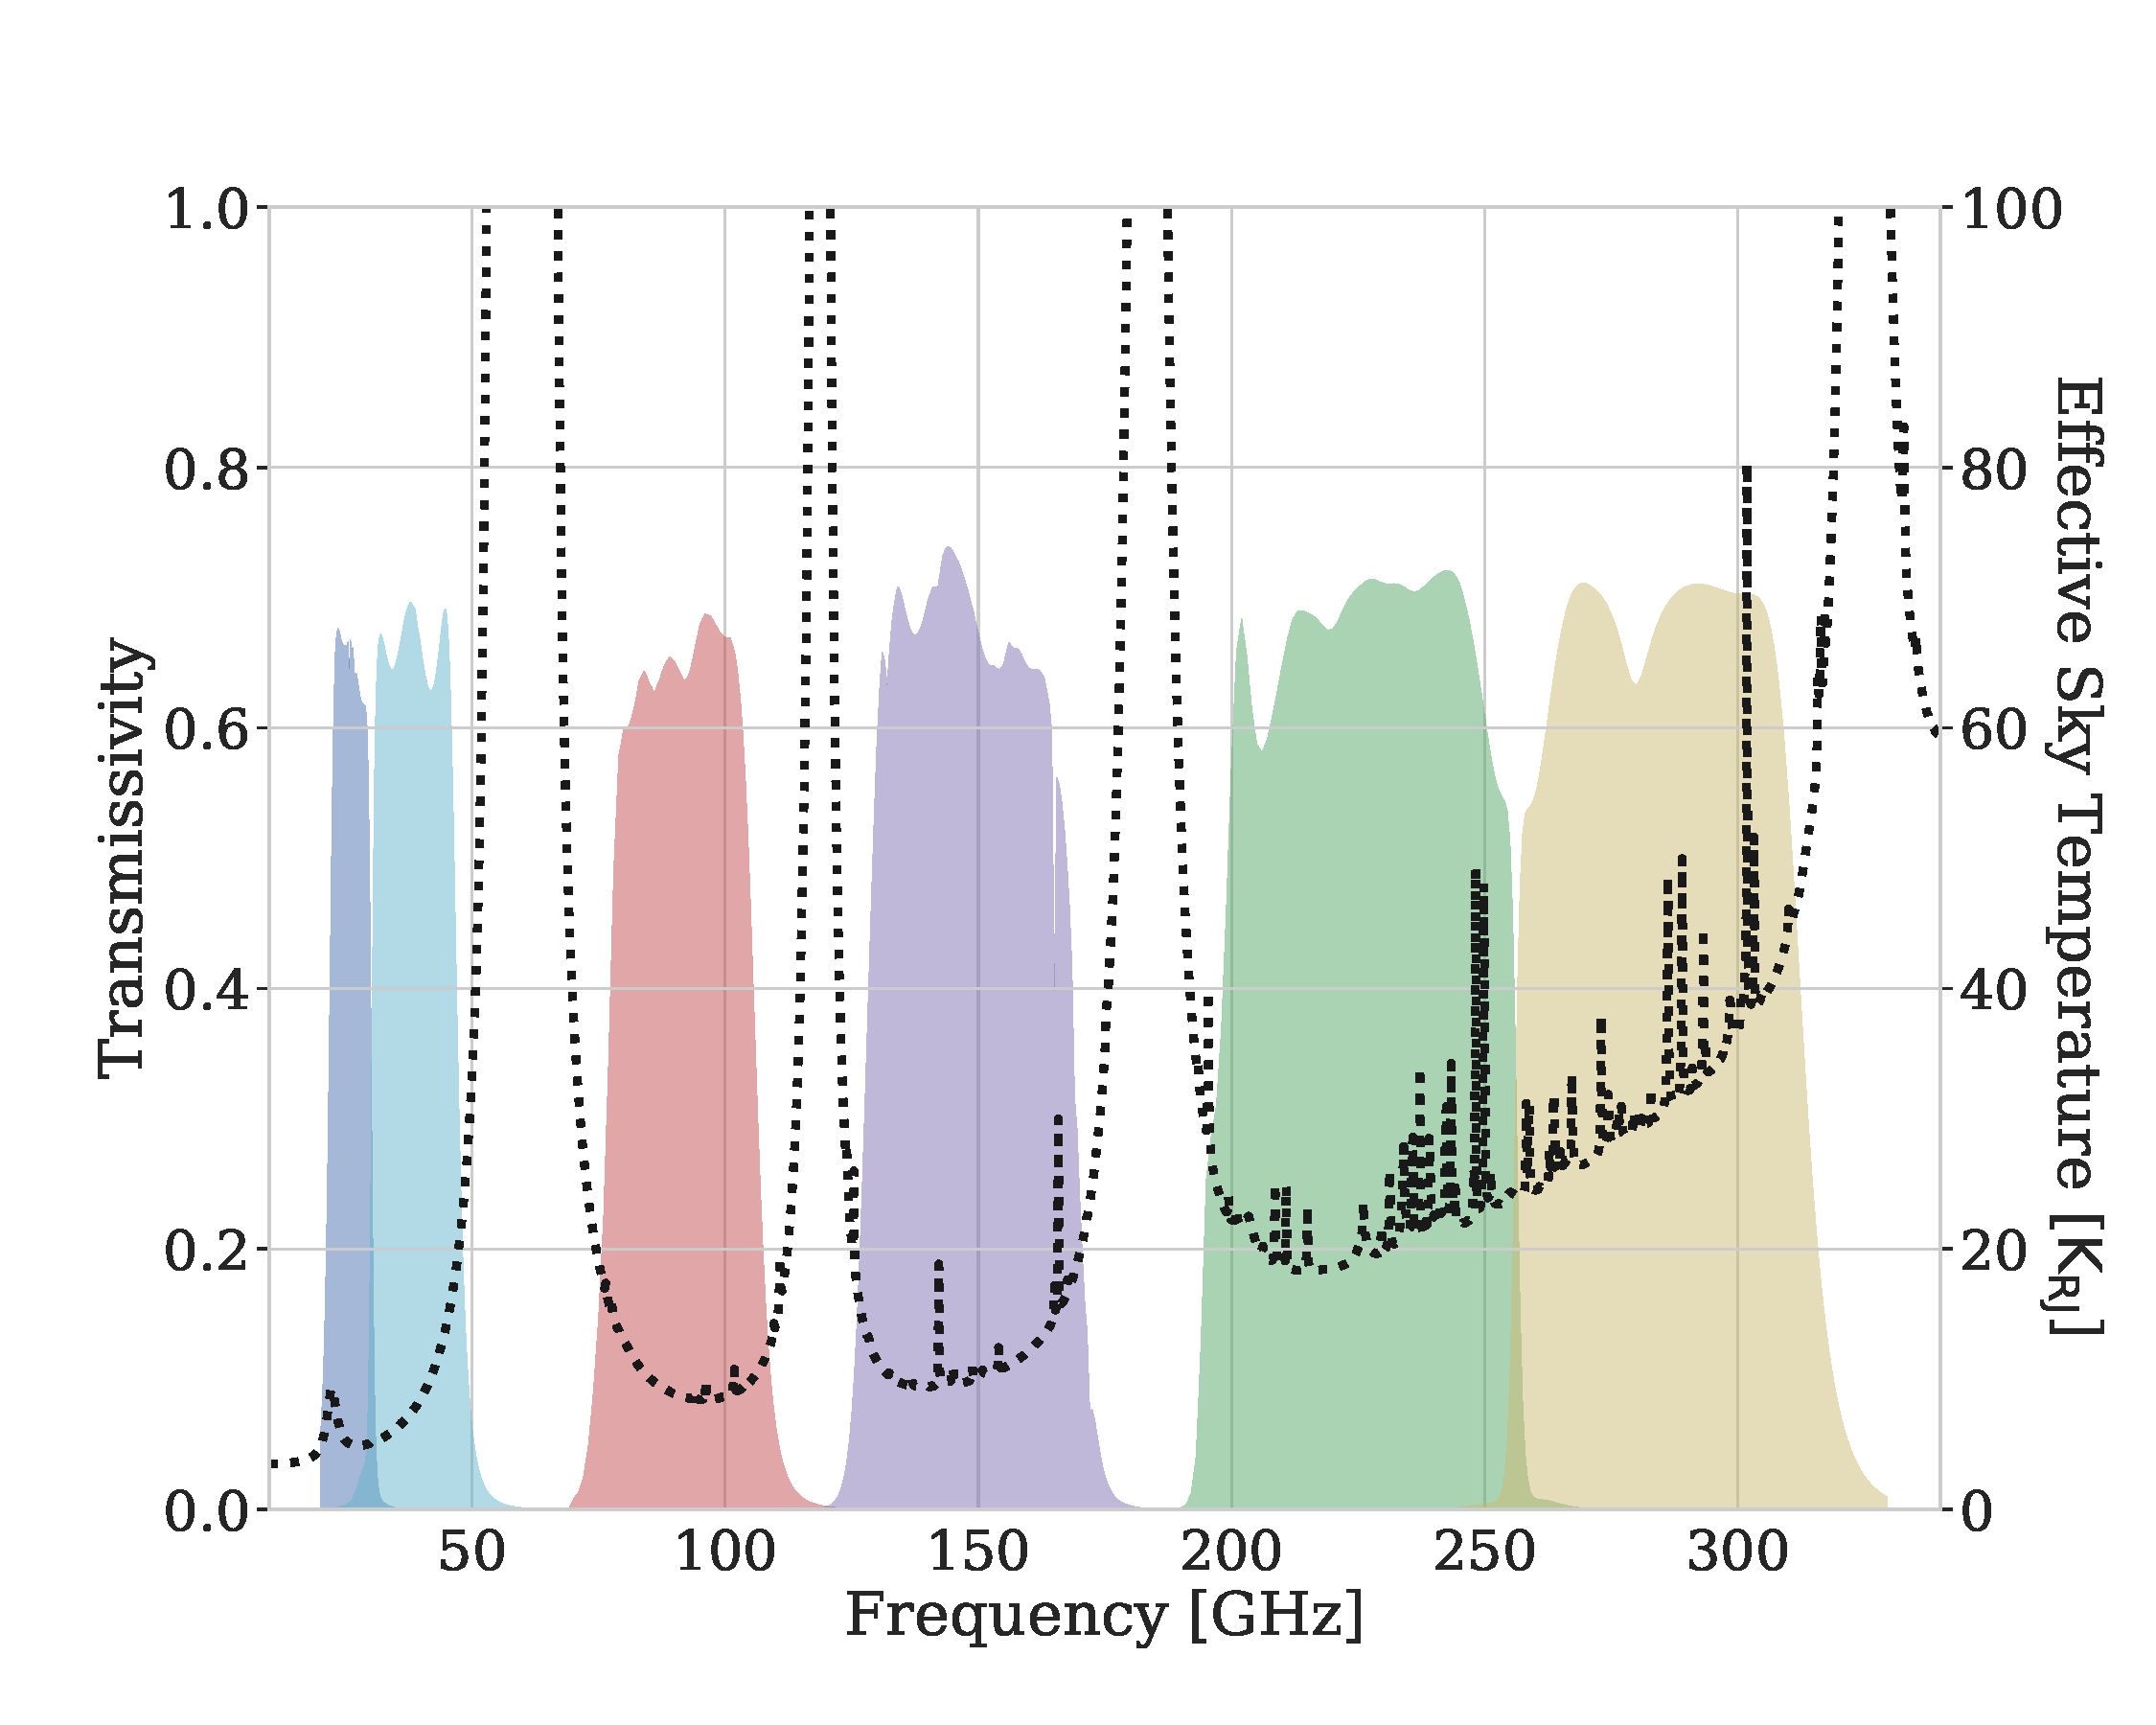
\includegraphics[width=0.8\linewidth, trim=0cm 1cm 0cm 2cm, clip]{InstrumentOverview/Figures/so_bands.pdf}
    \caption{The SO detector bands overplotted onto the Atacama sky's effective RJ temperature at 1.4~mm PWV and 50~deg elevation. The observation bands are placed in what are referred to as \important{atmospheric window} between the oxygen absorption/emission lines at $\sim$~60, 120, 180, and 330~GHz. The precipitous increase in atmospheric brightness temperature at high frequency is due to the increasing emissivity of water vapor in the far IR. This excess emission not only increases noise in the high-frequency bands but also increases the intensity the impact of atmospheric fluctuations, which makes 1/f noise mitigation challenging in the UHF bands.}
    \label{fig:so_bands_atacama}
\end{figure}

In order to quantify the amount of water in the atmosphere, we monitor the \textit{precipitable water vapor} (PWV), which is the height of liquid water equal to the amount of water vapor in an imaginary column from the ground to outer space. Emission due to water, and therefore the impact of PWV, increases with increasing frequency. To leading order, which applies reasonably well at low frequencies and small water composition, the sky intensity scales as
\begin{equation}
    T_{\mathrm{ATM}} \appropto \mathrm{PWV} \, .
    \label{eq:atmospheric_brightness_pwv_dependence}
\end{equation}
In practice, Equations~\ref{eq:atmospheric_brightness_elevation_dependence} and ~\ref{eq:atmospheric_brightness_pwv_dependence} are not used and are instead replaced by molecular simulations of the atmosphere's absorption and scattering profile, but these relations are nonetheless useful guides of water and oxygen's impact on atmospheric brightness. 

%%%%%%%%%%%%%%%%%%%%%%%%%%%%%%%%
%%%%%%%%%%%%%%%%%%%%%%%%%%%%%%%%

\subsection{Chile site}
\label{sec:sky_intensity}

\begin{figure}[!t]
    \centering
    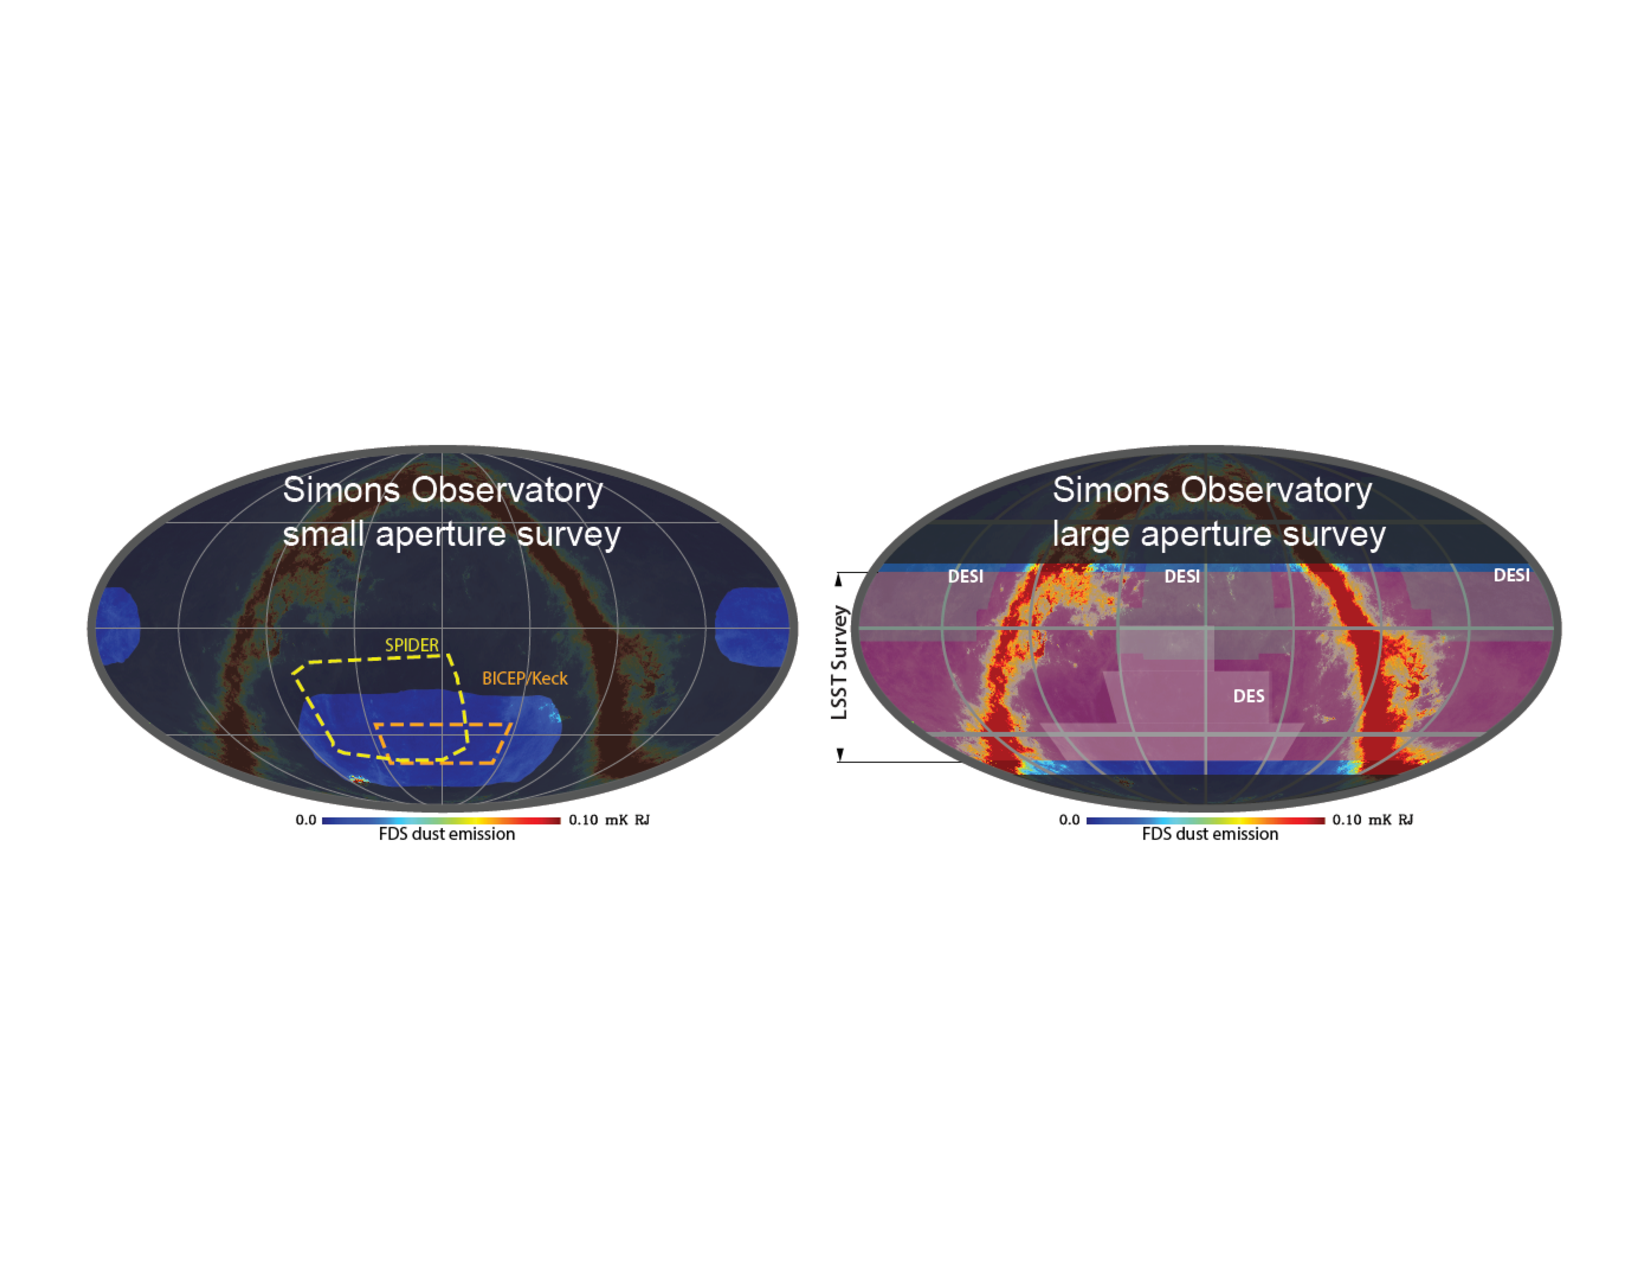
\includegraphics[width=\linewidth, trim=1cm 7cm 1cm 7cm, clip]{InstrumentOverview/Figures/so_survey.pdf}
    \caption{The LAT and SAT survey area for SO. The access to 70\% of the sky is a substantial advantage for the Atacama site compared to other sites, such as that at the South Pole.}
    \label{fig:so_survey}
\end{figure}

In order to minimize both the attenuation of the CMB and the parasitic photons due to the atmosphere, it is advantageous to observe through both as little and as dry of air as possible. The most effective approach to limit atmospheric power is to build a satellite and measure the CMB from beyond the Earth's atmosphere. While leaving Earth is certainly an effective technique to minimize the impact of its atmosphere, launching and operating a satellite costs $\sim$~billions of dollars and carries high risk, as the instrument cannot be serviced after launch. Despite these limitations, some of the most successful CMB instruments were satellite missions, including Planck and WMAP, which are discussed in Section~blah. Another effective strategy to avoid the atmosphere is to launch a high-altitude balloon, which can float at $\sim$~100,000~ft elevation, which is above $>$~99\% of the atmosphere. Though also an effective atmosphere-mitigation technique, balloons have observation lifetimes that are limited by their flight duration, and while they are much cheaper than satellites, they face the same challenges of not being able to fix the instrument after launch. For these practical reasons, observing the CMB from the ground is a competitive technique if you can do so from the right location.

\begin{figure}[!t]
    \centering
    \subfloat[\label{fig:site_photo}]{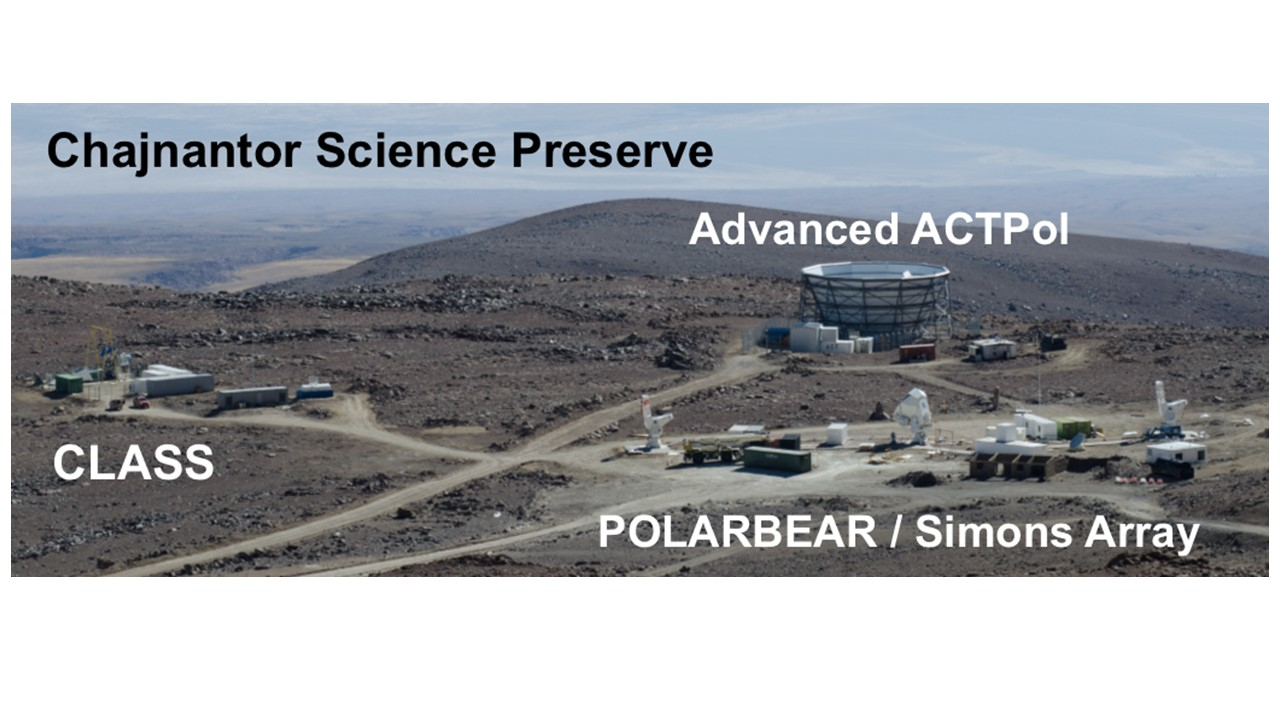
\includegraphics[width=\linewidth, trim=0cm 3.5cm 0cm 4cm clip]{InstrumentOverview/Figures/chajnantor_site.jpg}}
    \hfill
    \subfloat[\label{fig:pwv_distribution}]{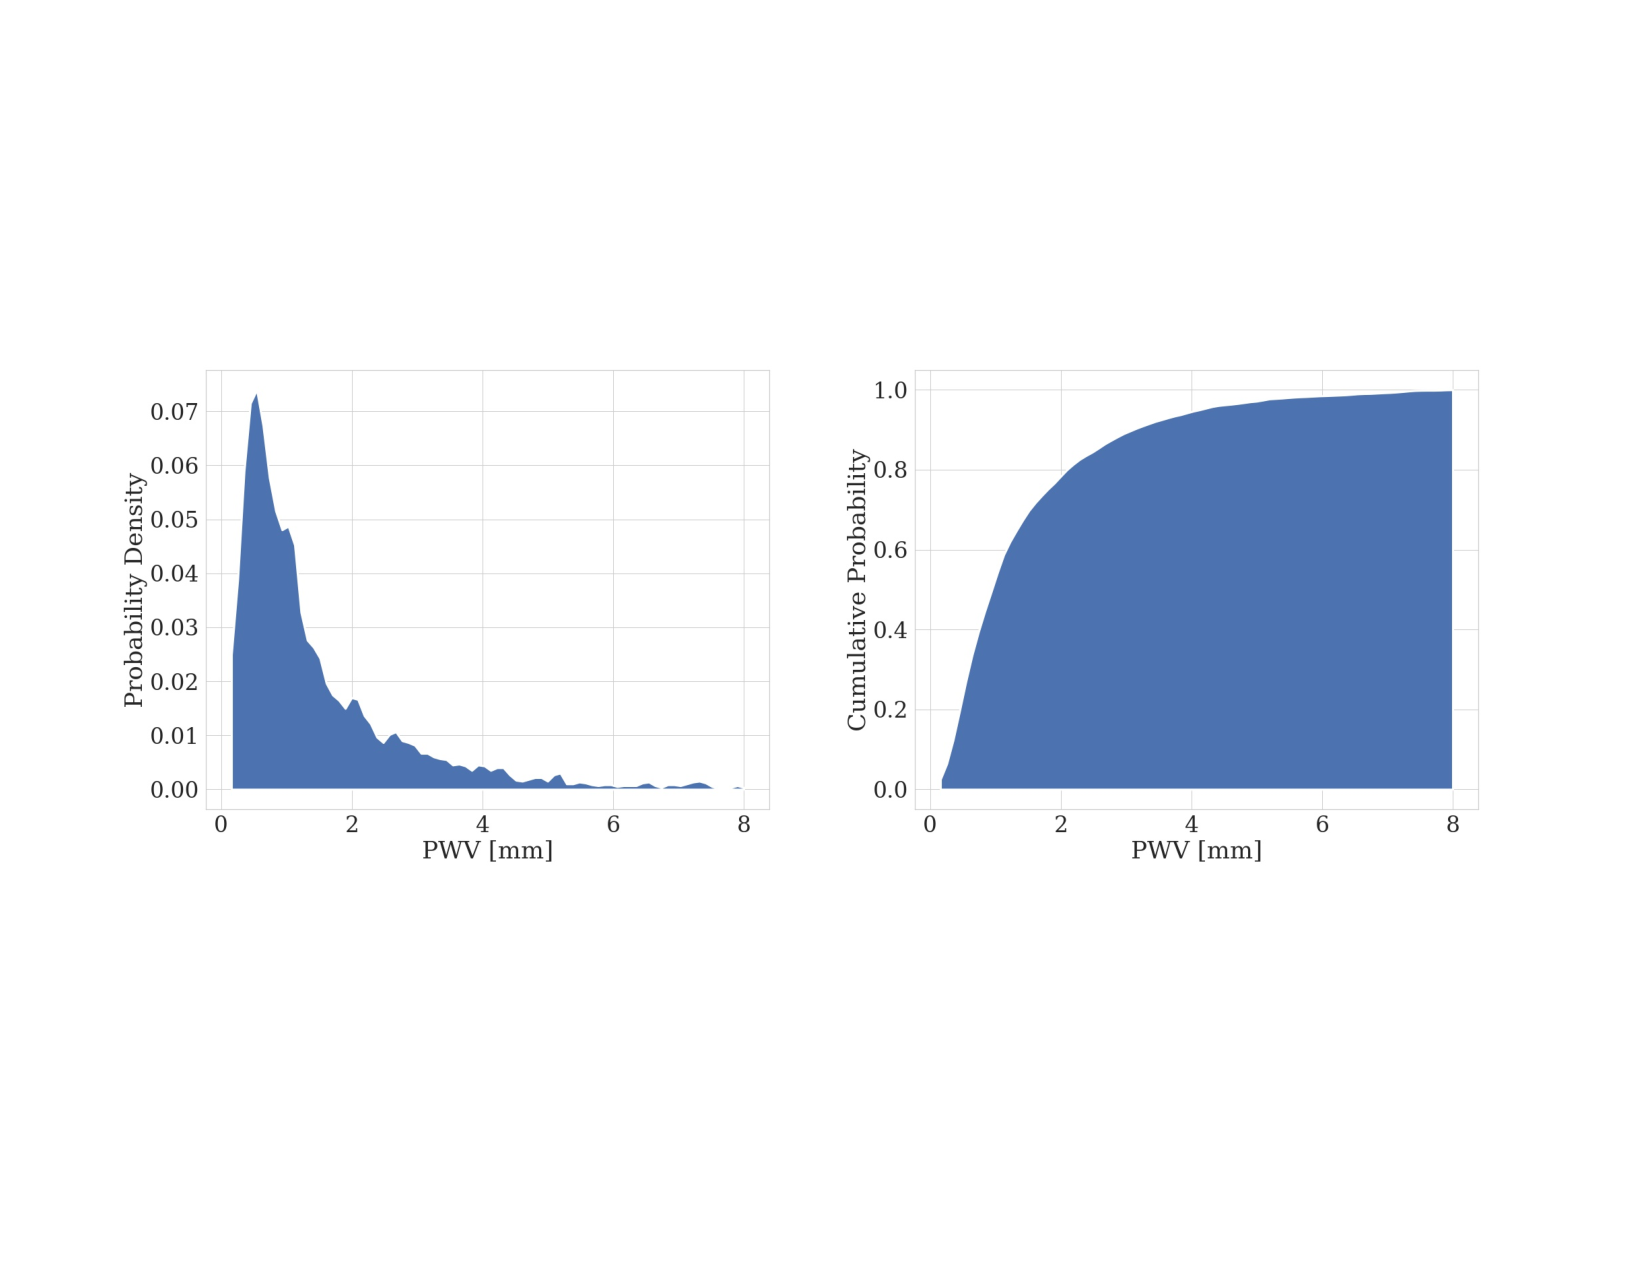
\includegraphics[width=0.95\linewidth, trim=2cm 7cm 3cm 6cm, clip]{InstrumentOverview/Figures/chile_pwv.pdf}}
    \caption[Chajnantor site]{Top panel: photograph of the observation site for Simons Array. Three PB2-style telescopes operate at 5,200 m elevation and neighbor Advanced ACT, CLASS, and Simons Observatory. PB2b operates on the southernmost of these three telescopes, which is furthest to the left. Figure courtesy of Nathan Stebor. Bottom panel: probability density and cumulative probability for PWV at the POLARBEAR-2 observation site. The median value is near 1 mm, where the value is below 2 mm nearly 80\% of the time. The dry conditions, combined with the thin atmosphere, make the Chajnantor site ideal for mm-wave astronomy observations.}
    \label{fig:pwv_distribution}
\end{figure}

Both SA and SO observe the CMB from the Chajnantor Science Preserve in the Atacama Desert of Chile on Cerro Toco. Located at 5,200~m elevation and in one of the most arid climates on Earth, Cerro Toco offers some of the best observing conditions that can be achieved terrestrially. Additionally, with its latitude of $\approx$~$-23^{\circ}$ has access to $>$~70\% of the sky, which in turn offers ample opportunity both to reduce cosmic variance by measuring a more angular modes (see Equation~\ref{eq:cosmic_variance}) and to cross correlate with other surveys. Also, because the sky rises, sets, and rotates during the course of the day in Chile, sky patches can easily be scanned in different directions---a technique called \important{cross linking}---which is a powerful tool to mitigate scan-dependent systematic errors. These last two characteristics are in contrast to another widely-used CMB observation site, the South Pole, which has access to a smaller fraction of the sky and offers no sky rotation. Figure shows the location of the Chile observation site, as well as a recent photograph of the Chilean observational site. Neighboring to SA and SO are the Atacama Cosmology Telescope (ACT) and the Cosmology Large Angular Scale Surveyor (CLASS).

Figure~\ref{fig:pwv_distribution} shows a probability distribution of the PWV during PB-1's second observation season. The median is near 1~mm, and for reference, the annual median PWV for Portland, Oregon is 20~mm, demonstrating that indeed, high-elevation, desert conditions of the Chilean observation site is indeed quite dry.

%%%%%%%%%%%%%%%%%%%%%%%%%%%%%%%%
%%%%%%%%%%%%%%%%%%%%%%%%%%%%%%%%
%%%%%%%%%%%%%%%%%%%%%%%%%%%%%%%%

\section{Optics}
\label{sec:simons_array_optics}

In its simplest form, the purpose of a CMB telescope is to image the sky onto an array of detectors with low distortion and high throughput, all while introducing minimal parasitic loading. Because 100~GHz optics are no widely available in the private sector, CMB telescopes are custom designed using unique materials that have favorable optical properties at microwave frequencies. In addition, in order to minimize photon loading, CMB optical systems are cooled to cryogenic temperatures, which both improves their transparency and limits their thermal emission. In this section, we overview the elements of the SA and SO optical systems that are relevant to the research presented in this thesis. We start by discussing SA in detail, and then we formulate a discussion of the SO optics by highlighting its differences to that of SA.

There are many figures of merit when evaluating an optical system, including field of view,  angular resolution, optical efficiency, magnification/plate scale, and (polarized) image fidelity. While each of these is important and interesting, the following subsections will focus only on what is relevant to the primary research of this thesis. 

%%%%%%%%%%%%%%%%%%%%%%%%%%%%%%%%
%%%%%%%%%%%%%%%%%%%%%%%%%%%%%%%%

\subsection{Telescope and receiver optics}
\label{sec:telescope_optics}

The SA telescope is shown as part of Figure~\ref{fig:pb2_telescope} and is composed of two monolithic mirrors that together form an off-axis Gregorian configuration. The primary mirror is a parabolic reflector that focuses incoming parallel rays onto the \textit{prime focus}. The image at prime focus is diffraction limited over only a small field of view and is therefore reimaged by an ellipsoidal secondary mirror onto the \textit{Gregorian focus}. While improved with respect to that of the primary mirror, this focus is not telecentric and still has only a moderate diffraction-limited field of view (FOV), and therefore a \textit{receiver cryostat} (also often referred to as the \textit{camera}) is employed to reimage the telescope image onto the detector array. The telescope mirrors are part of a compact telescope assembly, a photo of which is shown in Figure~\ref{fig:pb2_telescope}, which is designed to be nimble in order to enable more flexibility (speed, acceleration, elevation range, etc.) in how sky patches are scanned.

The advantages of the off-axis Gregorian design are its compactness and its satisfying the \important{Mizuguchi-Dragone} condition, which limits cross polarization by correcting any polarization rotation on the primary mirror with the secondary. The disadvantages of the SA telescope are that its mirrors are at ambient temperatures, which necessitates tight control of stray light to limit the number of 300~K photons that travel into the receiver, and that the off-axis design induces intensity to polarization (I-to-P) leakage along the y direction due to the finite conductivity of the mirror's metal, which is a systematic effect that must be subtracted from the detector data.

The SA receiver cryostat, which is also shown in Figure~\ref{fig:pb2_telescope}, contains three reimaging lenses: the field lens, aperture lens, and collimator lens. The field lens is effectively responsible for adjusting the speed of the optics at secondary focus, while the aperture and collimator lenses form an image of the primary mirror at the \textit{Lyot stop} while also forming a high-fidelity, telecentric, large-field-of-view sky image at the focal plane. All three lenses are made of alumina, which is sintered/amorphous aluminum oxide $\mathrm{Al_{2}O_{3}}$ with a high index or refraction in mm-wave ($n \approx 3.1$), and are cooled to $\approx$~4~K.

\begin{figure}
    \centering
    \subfloat[\label{fig:pb2_telescope_photo}]{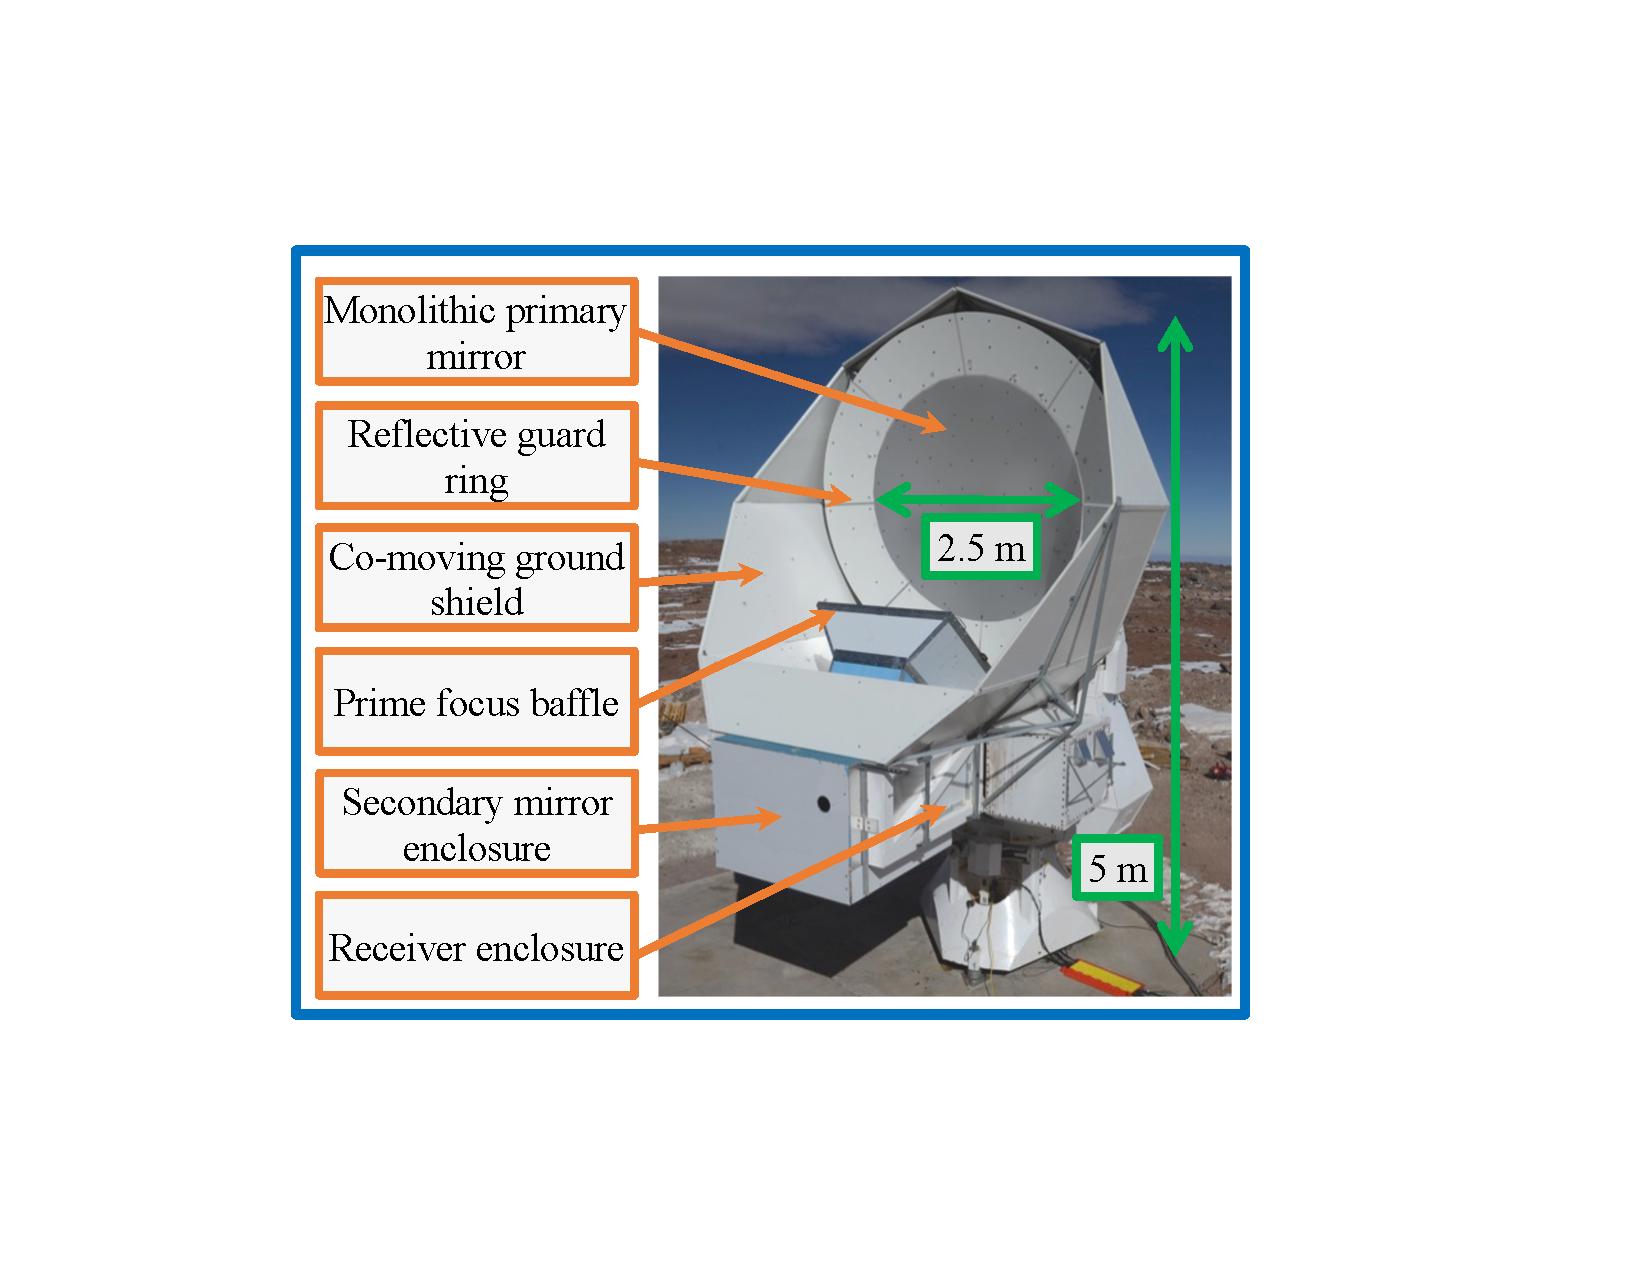
\includegraphics[width=0.9\linewidth, trim=0cm 4cm 0.5cm 4cm, clip]{InstrumentOverview/Figures/PB2b_telescope.pdf}}
    \hfill
    \subfloat[\label{fig:pb2_telescope_cad}]{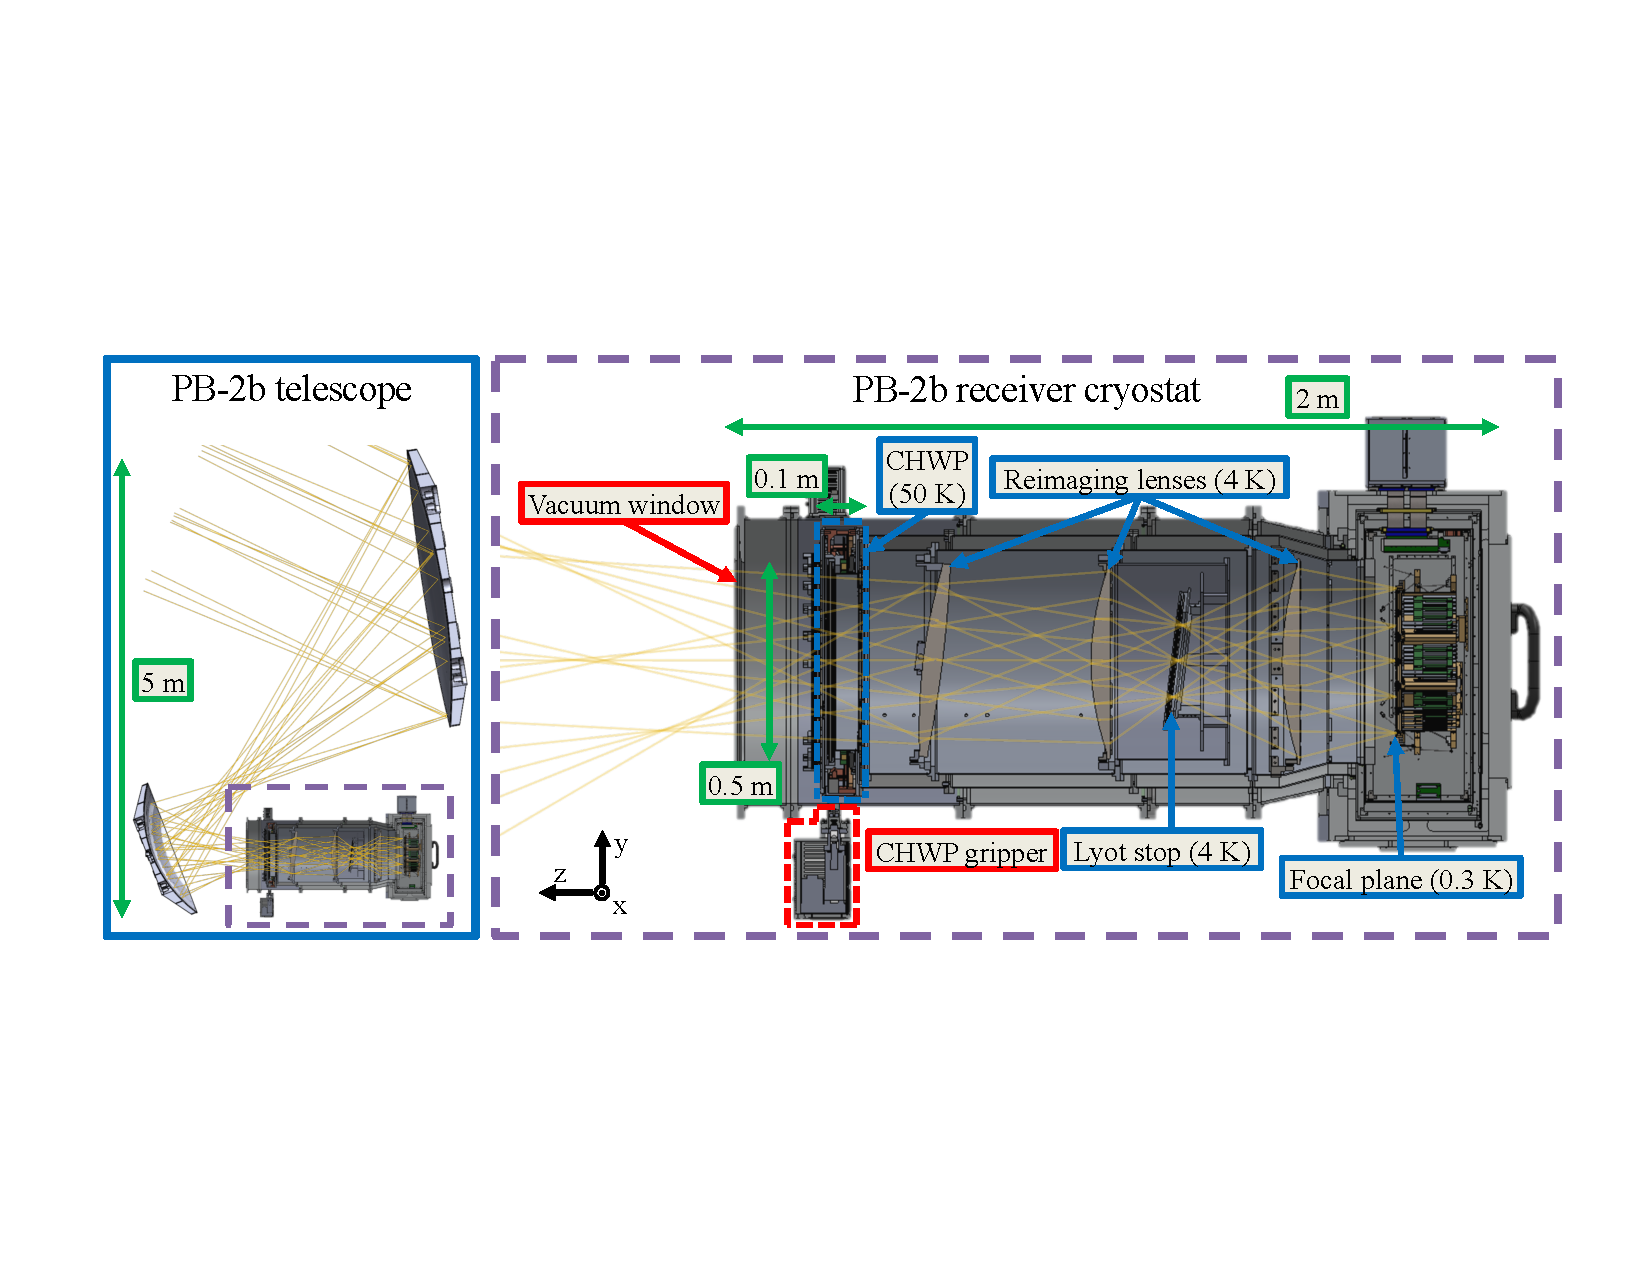
\includegraphics[width=\linewidth, trim=1.5cm 5.5cm 1.5cm 6cm, clip]{InstrumentOverview/Figures/PB2b_telescope_receiver.pdf}}
    \caption[POLARBEAR-2 telescope]{Photograph of the POLARBEAR-2 telescope. The primary and secondary mirros for an off-axis Gregorian pair. The primary reflector has a diameter of 3 m, which provides arcminute-scale angular resolution, but the compact design allows for relatively easy telescope motion. This unique combination of a large reflector and compact telescope provides POLARBEAR-2 with observational versatiliy.}
    \label{fig:pb2_telescope}
\end{figure}

The SO telescopes are shown in Figure~\ref{fig:so_telescope} and are of two varieties: a large-aperture telescope (LAT) and a small-aperture telescope (SAT). The LAT is composed of two paneled mirrors (not monolithic) which together form a crossed Dragone configuration. While less compact than the off-axis Gregorian that SA uses, the crossed Dragone (CD) offers many appealing optical properties, including outstanding image quality over a large field of view. For this reason, some small aperture telescopes in the CMB field use a CD optical system re-imaging optics. SO does, however, employ the LAT receiver cryostat (LATR) to re-image the LAT focus onto an array of up to 13 discrete focal planes, each with its own optics tube (OT). In order to push the limits of the FOV, each optics tube uses an alumina wedge that corrects the wavefront at the start of each OT such that the chief ray is approximately parallel to each OT's boresight. Then, three silicon reimaging lenses at 1~$\sim$~4~K re-image onto a detector array, through a Lyot stop, in a similar manner to the SA receiver.

The SO SAT is designed only to measure large-angular-scale CMB fluctuations, and therefore it has a smaller aperture than that of the SA and SO large-aperture telescopes. Its aperture stop is at $\sim$~2~K and is located near the vacuum window. The imaging optics comprise three silicon lenses at 1~$\sim$~2~K which image onto a $\approx$~400~mm diameter focal plane. This simpler design is much cheaper than the LAT, enabling four SATs to be constructed and operated in parallel.

\begin{figure}
    \centering
    \subfloat[\label{fig:lat_cad}]{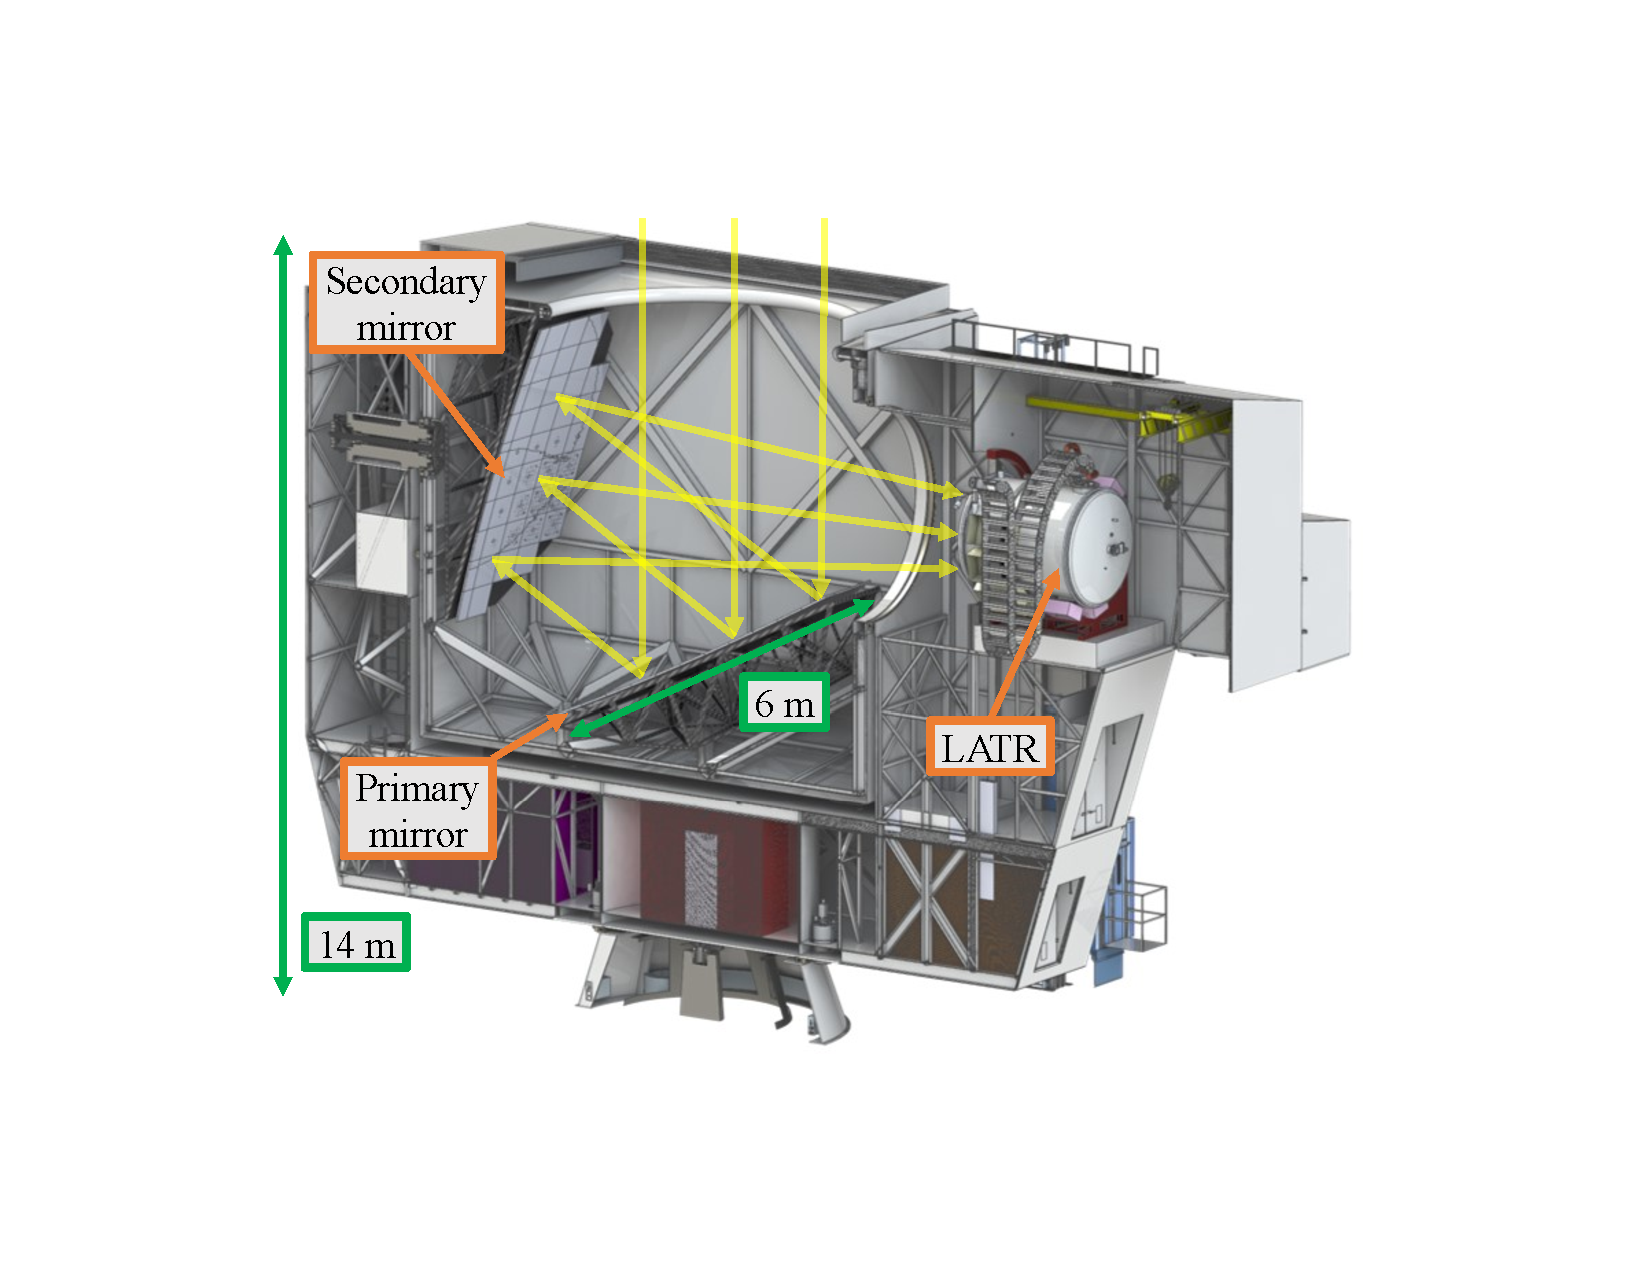
\includegraphics[width=0.7\linewidth, trim=3cm 3cm 3cm 3cm, clip]{InstrumentOverview/Figures/lat_cad.pdf}}
    \hfill
    \subfloat[\label{fig:lat_cad}]{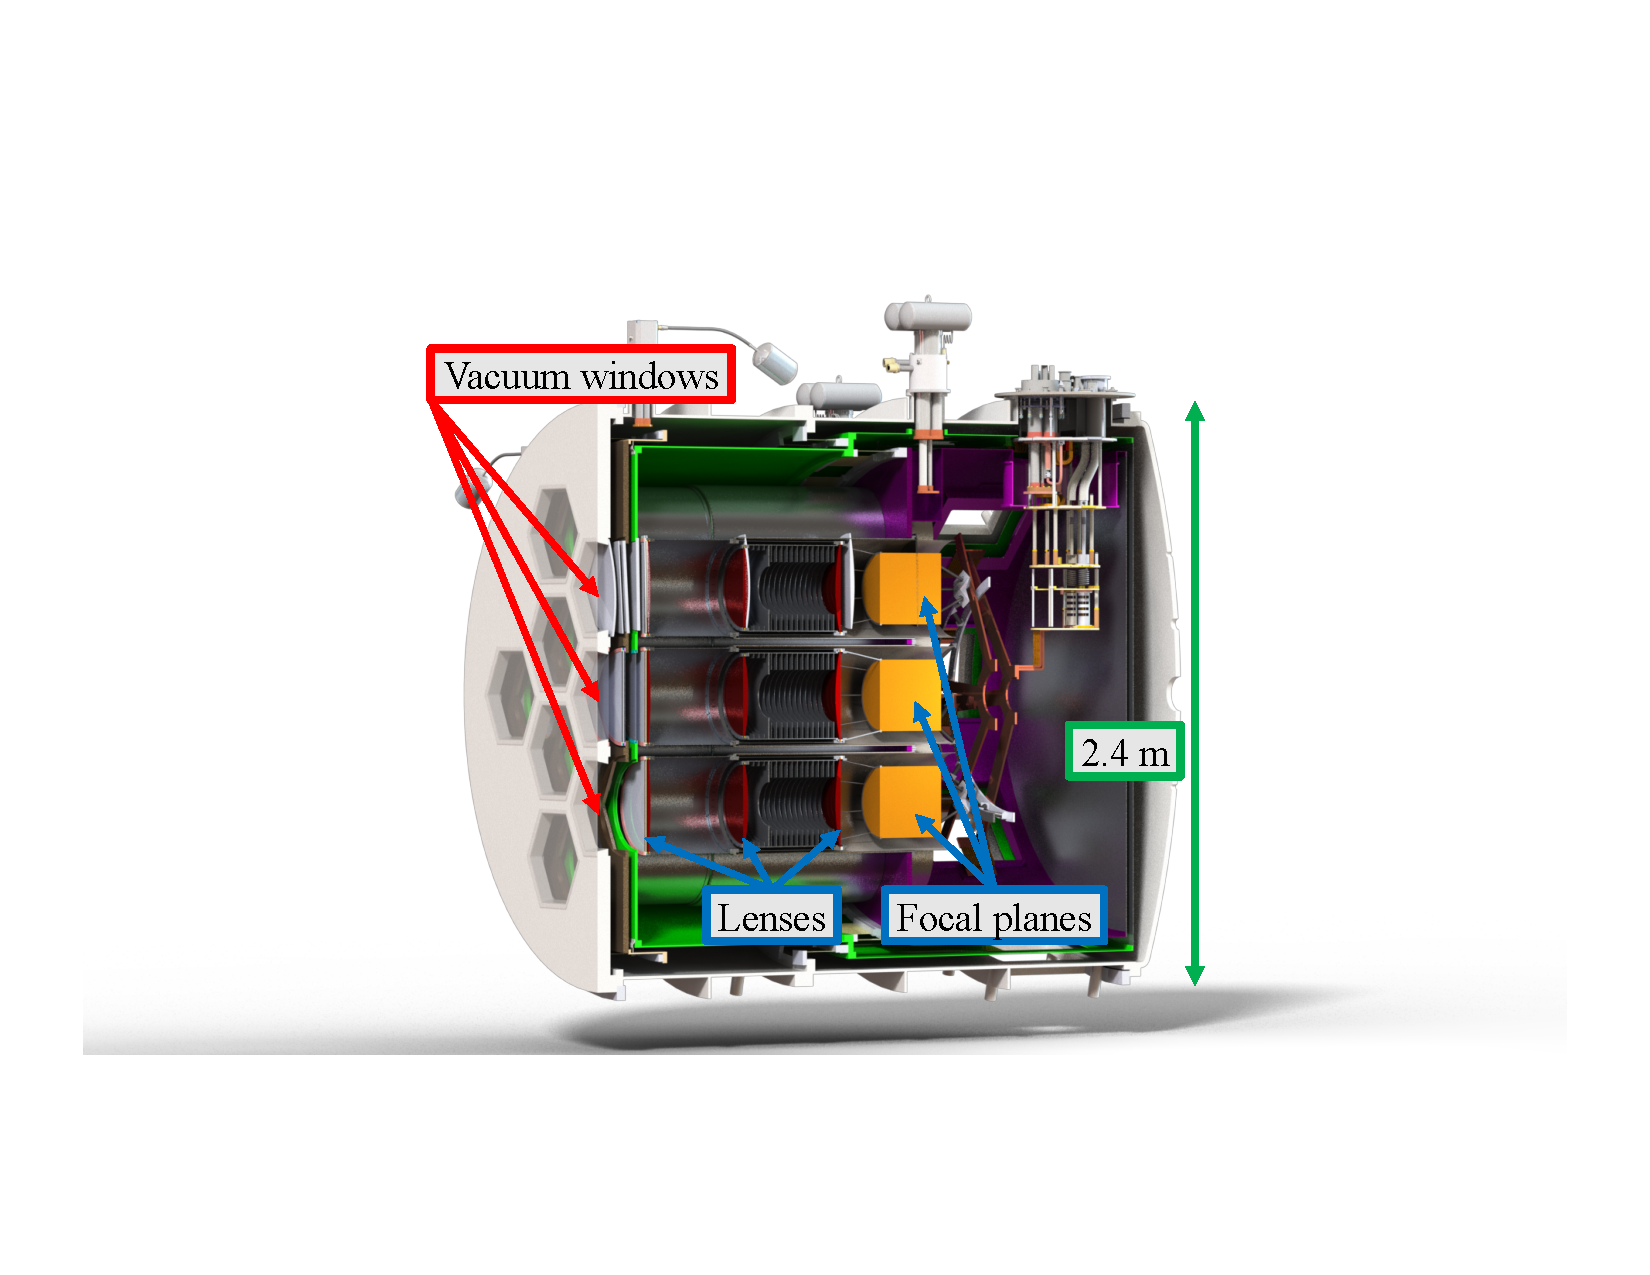
\includegraphics[width=0.5\linewidth, trim=7cm 4cm 7cm 5cm, clip]{InstrumentOverview/Figures/latr_cad.pdf}}
    \subfloat[\label{fig:lat_cad}]{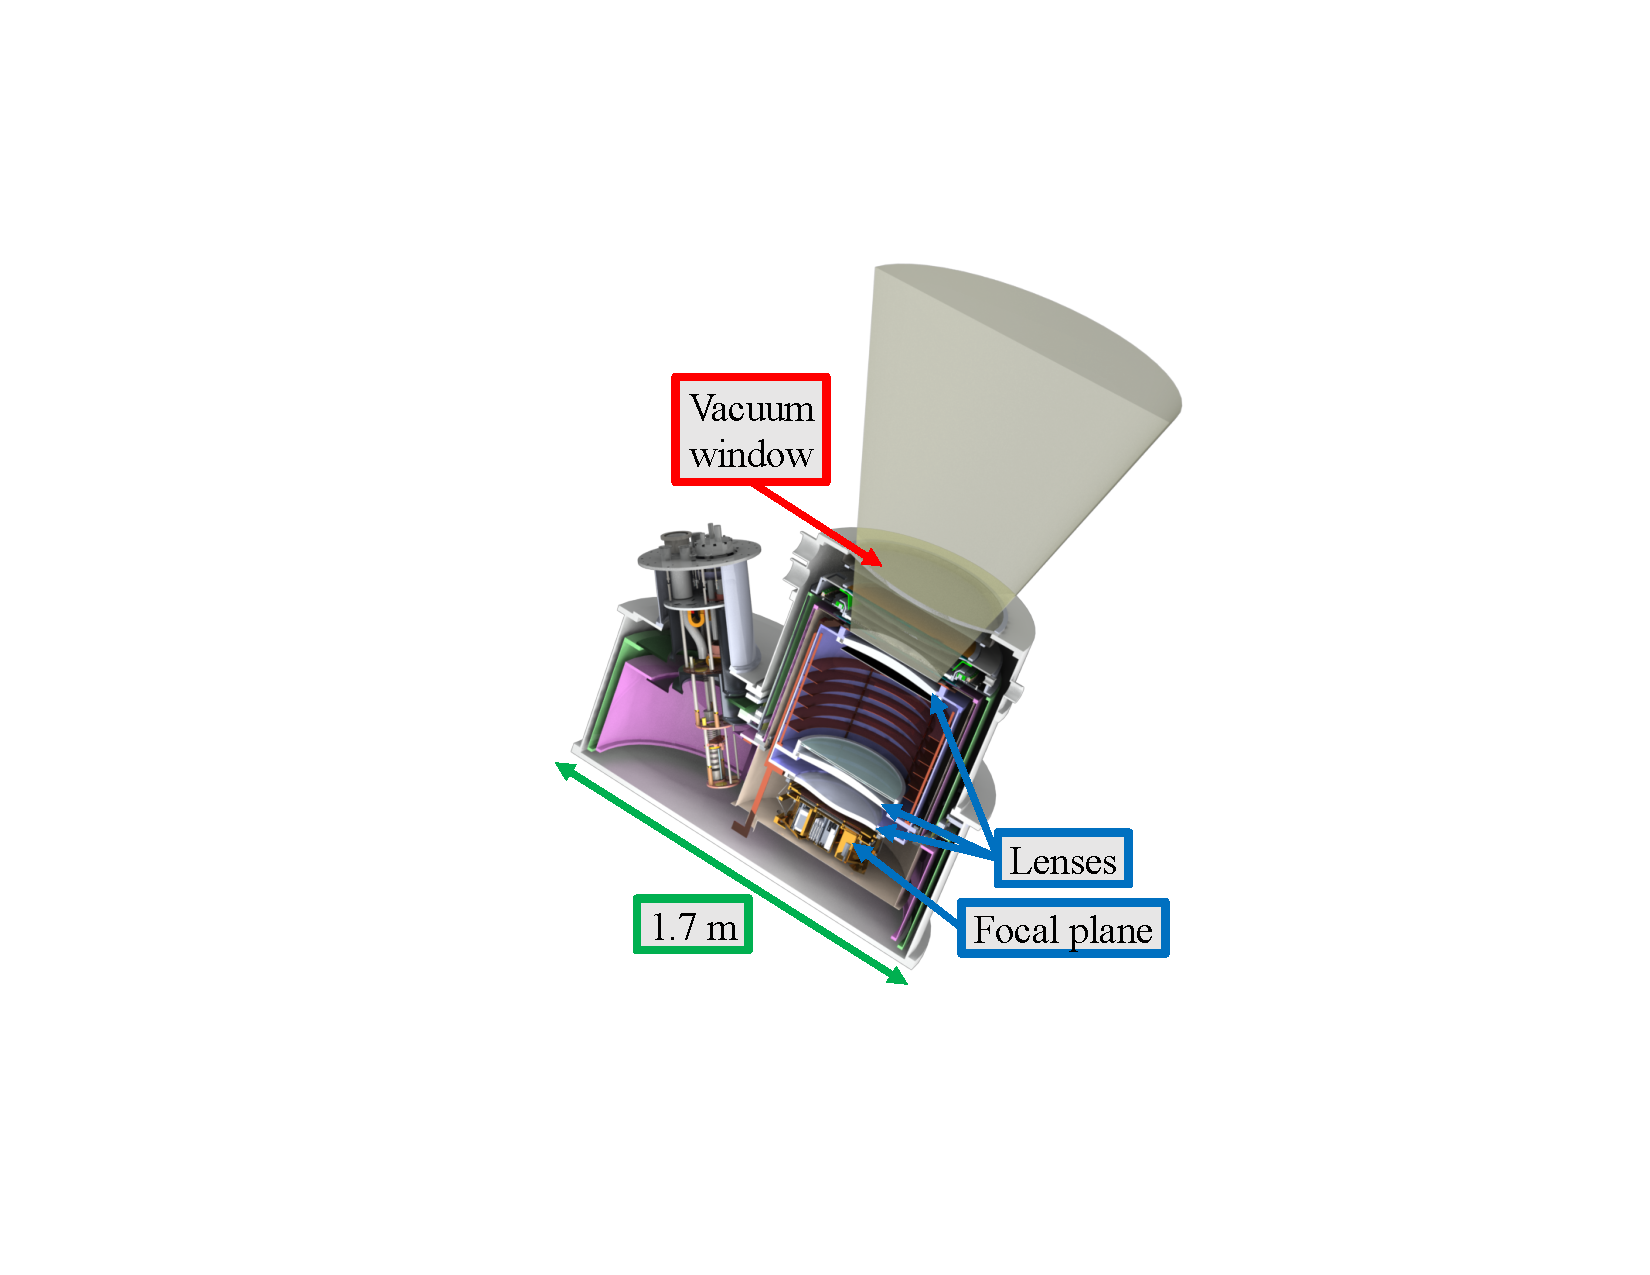
\includegraphics[width=0.5\linewidth, trim=7cm 5cm 7cm 4cm, clip]{InstrumentOverview/Figures/sat_cad.pdf}}
    \caption{Caption}
    \label{fig:so_telescope}
\end{figure}

All SA receivers and all SO SATs employ sapphire continuously-rotating half-wave plate (HWP) polarization modulators. The SA HWPs are located near the receiver's vacuum window, which is near the telescopes Gregorian focus, while the SO SAT HWPs are located directly in front of the aperture stop. HWPs are are a powerful tool to modulate sky polarization while rejecting the unpolarized atmosphere, which in turn suppresses atmospheric low-frequency noise and enables improved sensitivity to large angular scale modes. HWPs are a central research topic of this thesis document, and therefore we forego details here for a comprehensive discussion in Chapters~blah.

The most important shared characteristics of the SA and SO telescopes systems is that they are diffraction limited and FOV limited, that each receiver and optics tube images the sky onto the focal plane with high image fidelity and telecentricity, and that the diffraction-limited throughput of the system is limited by the aperture stop (or, more specifically for the SA and SO LAT, the Lyot stop). These properties are underlying assumptions for many of the calculations in Chapters to follow and are a good approximation for the presented telescope designs.

%%%%%%%%%%%%%%%%%%%%%%%%%%%%%%%%
%%%%%%%%%%%%%%%%%%%%%%%%%%%%%%%%

\subsection{Focal plane optics}
\label{sec:focal_plane_optics}

As discussed in the previous section, the telescope and receiver cryostat optics image the sky onto a focal plane. The job of the focal plane optics is to then couple the telescope image to detectors. The focal plane is comprised of discrete \important{detector pixels}, each of which is sensitive to two polarizations and two colors. PB-2a, PB-2b, two SATs, and some LAT OTs observe at 90 and 150~GHz (MF), PB-2c, one SAT, and some other LAT OTs observe at 220 and 270~GHz (UHF), and one SAT and the remaining LAT OTs observe at 30 and 40~GHz (LF).  Given this configuration, the goal of the focal plane optics is to achieve high throughput across broad bandwidths while also limiting out-of-band power.

\begin{figure}[!t]
    \centering
    \subfloat[\label{fig:focal_plane_optics:a}]{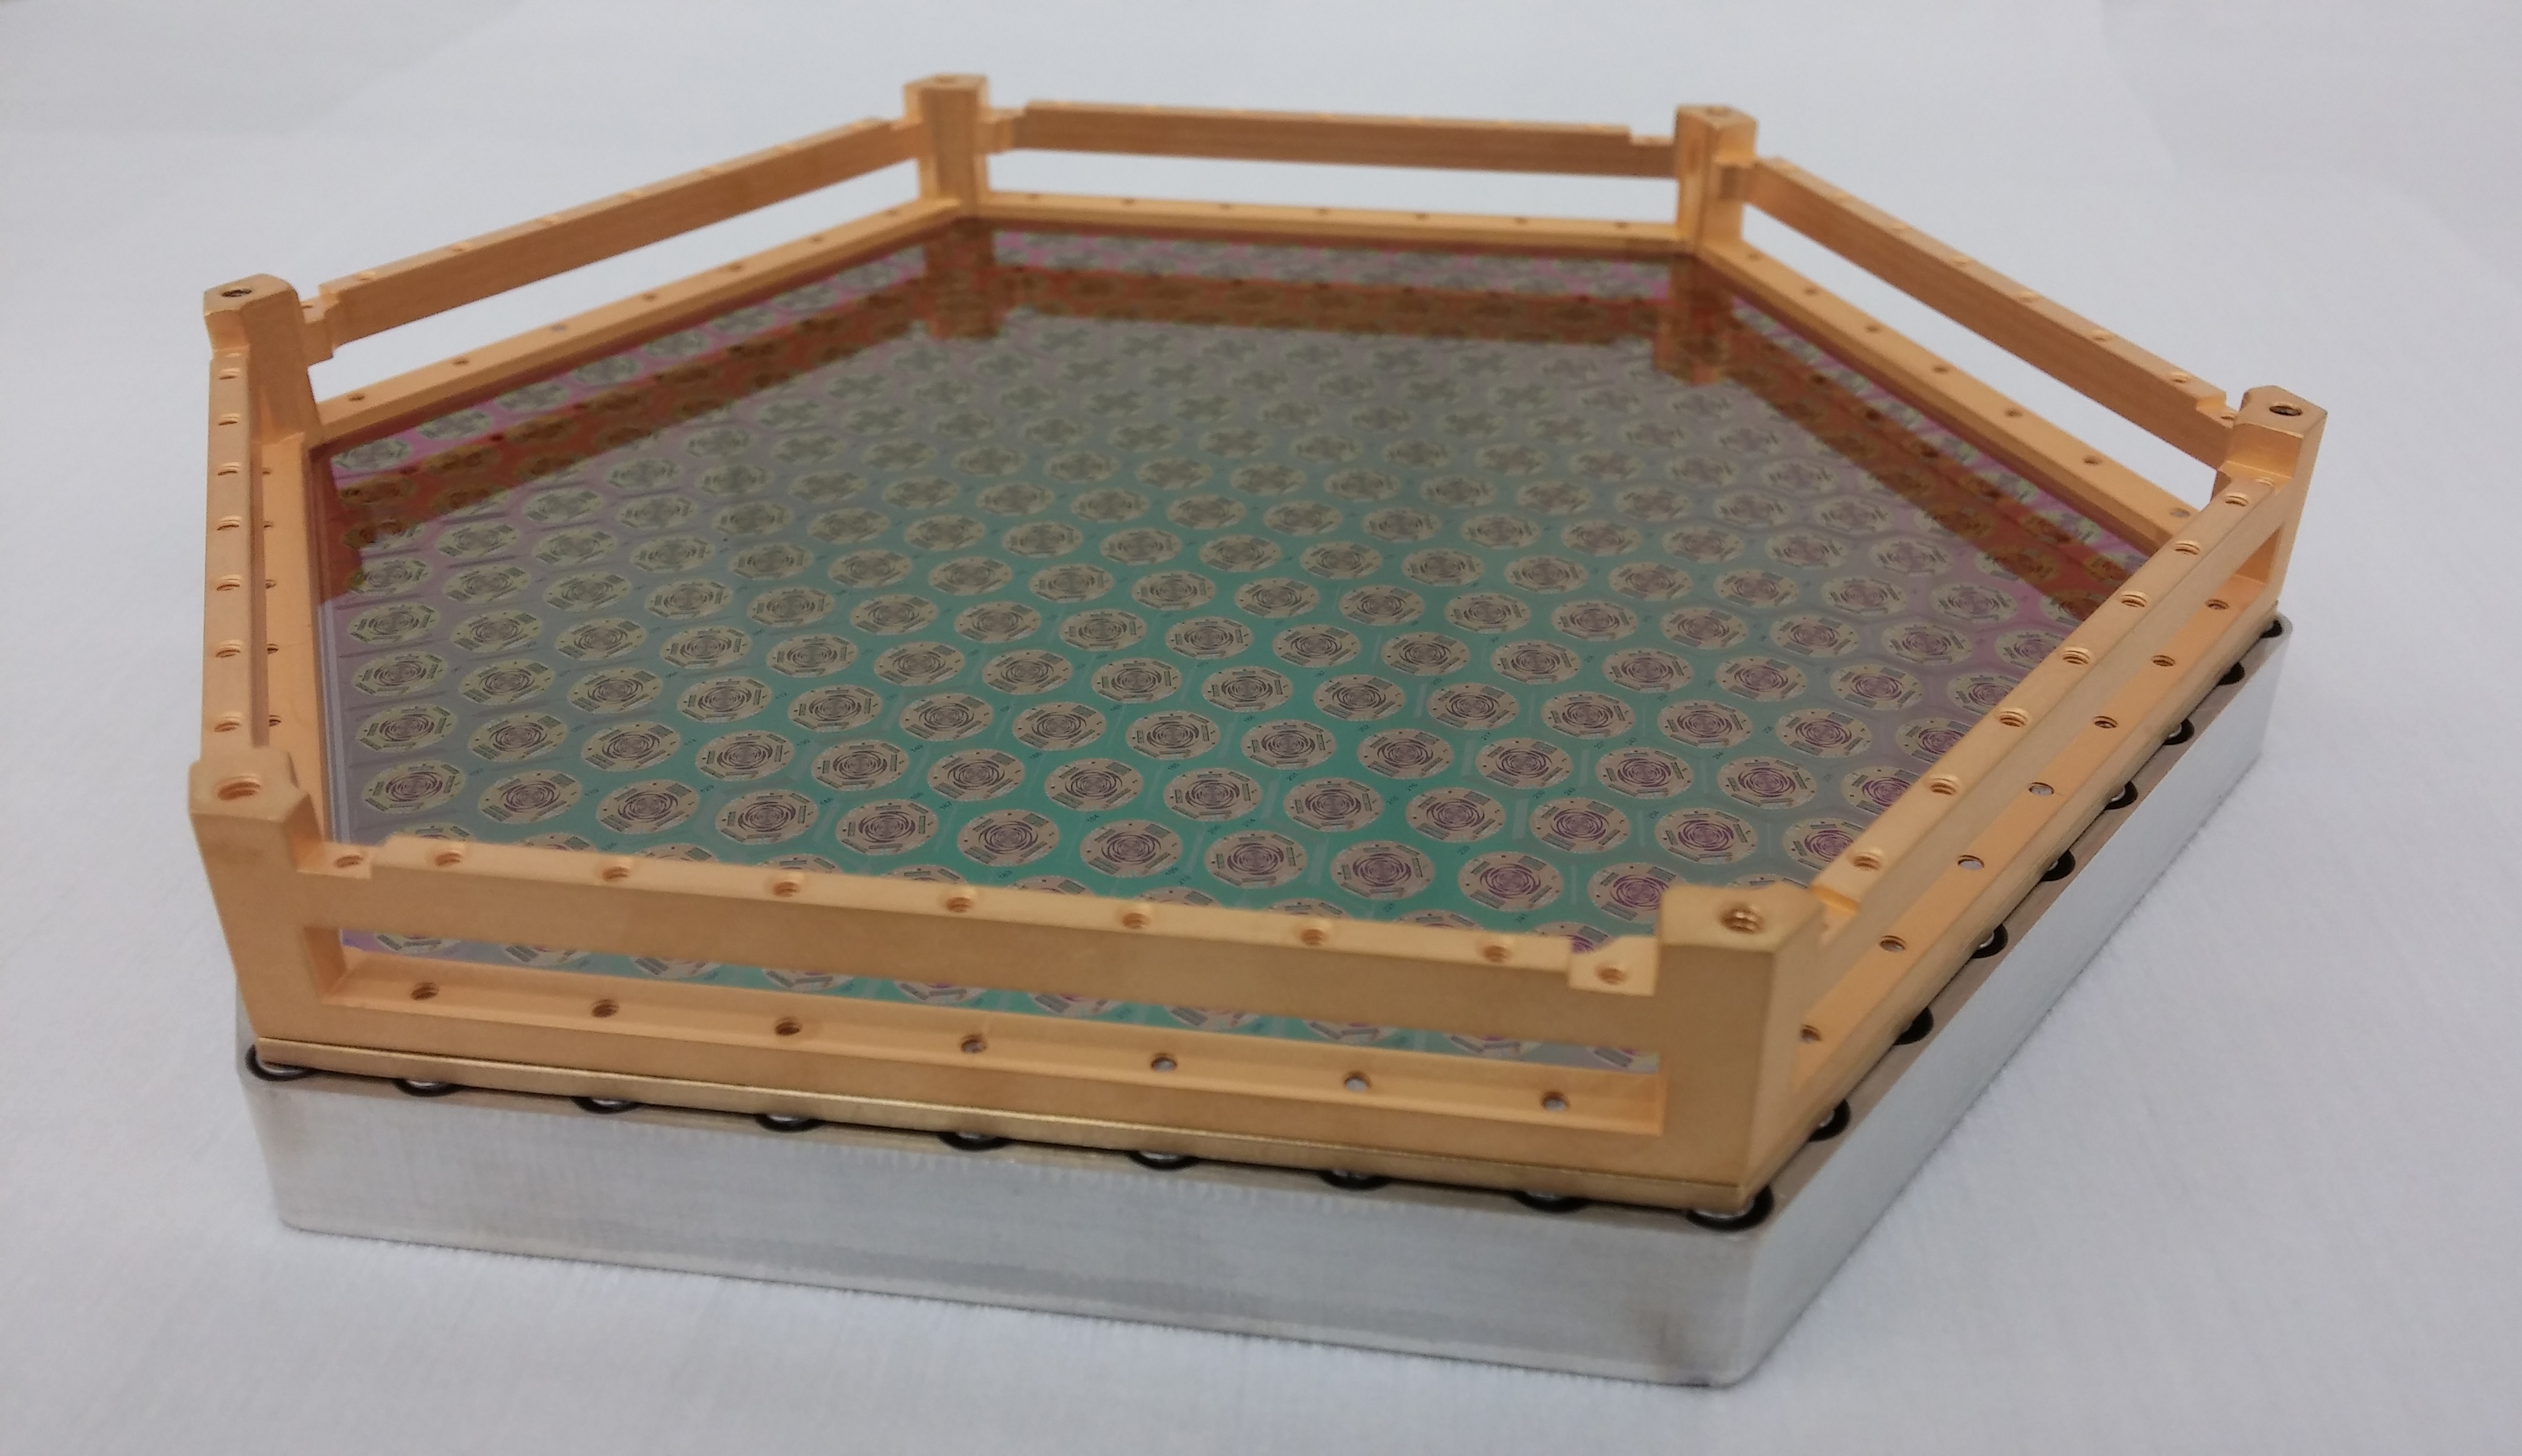
\includegraphics[width=0.48\linewidth, trim=0cm 0cm 0cm -0.2cm, clip]{InstrumentOverview/Figures/PB2_antennas.jpg}}
    \subfloat[\label{fig:focal_plane_optics:b}]{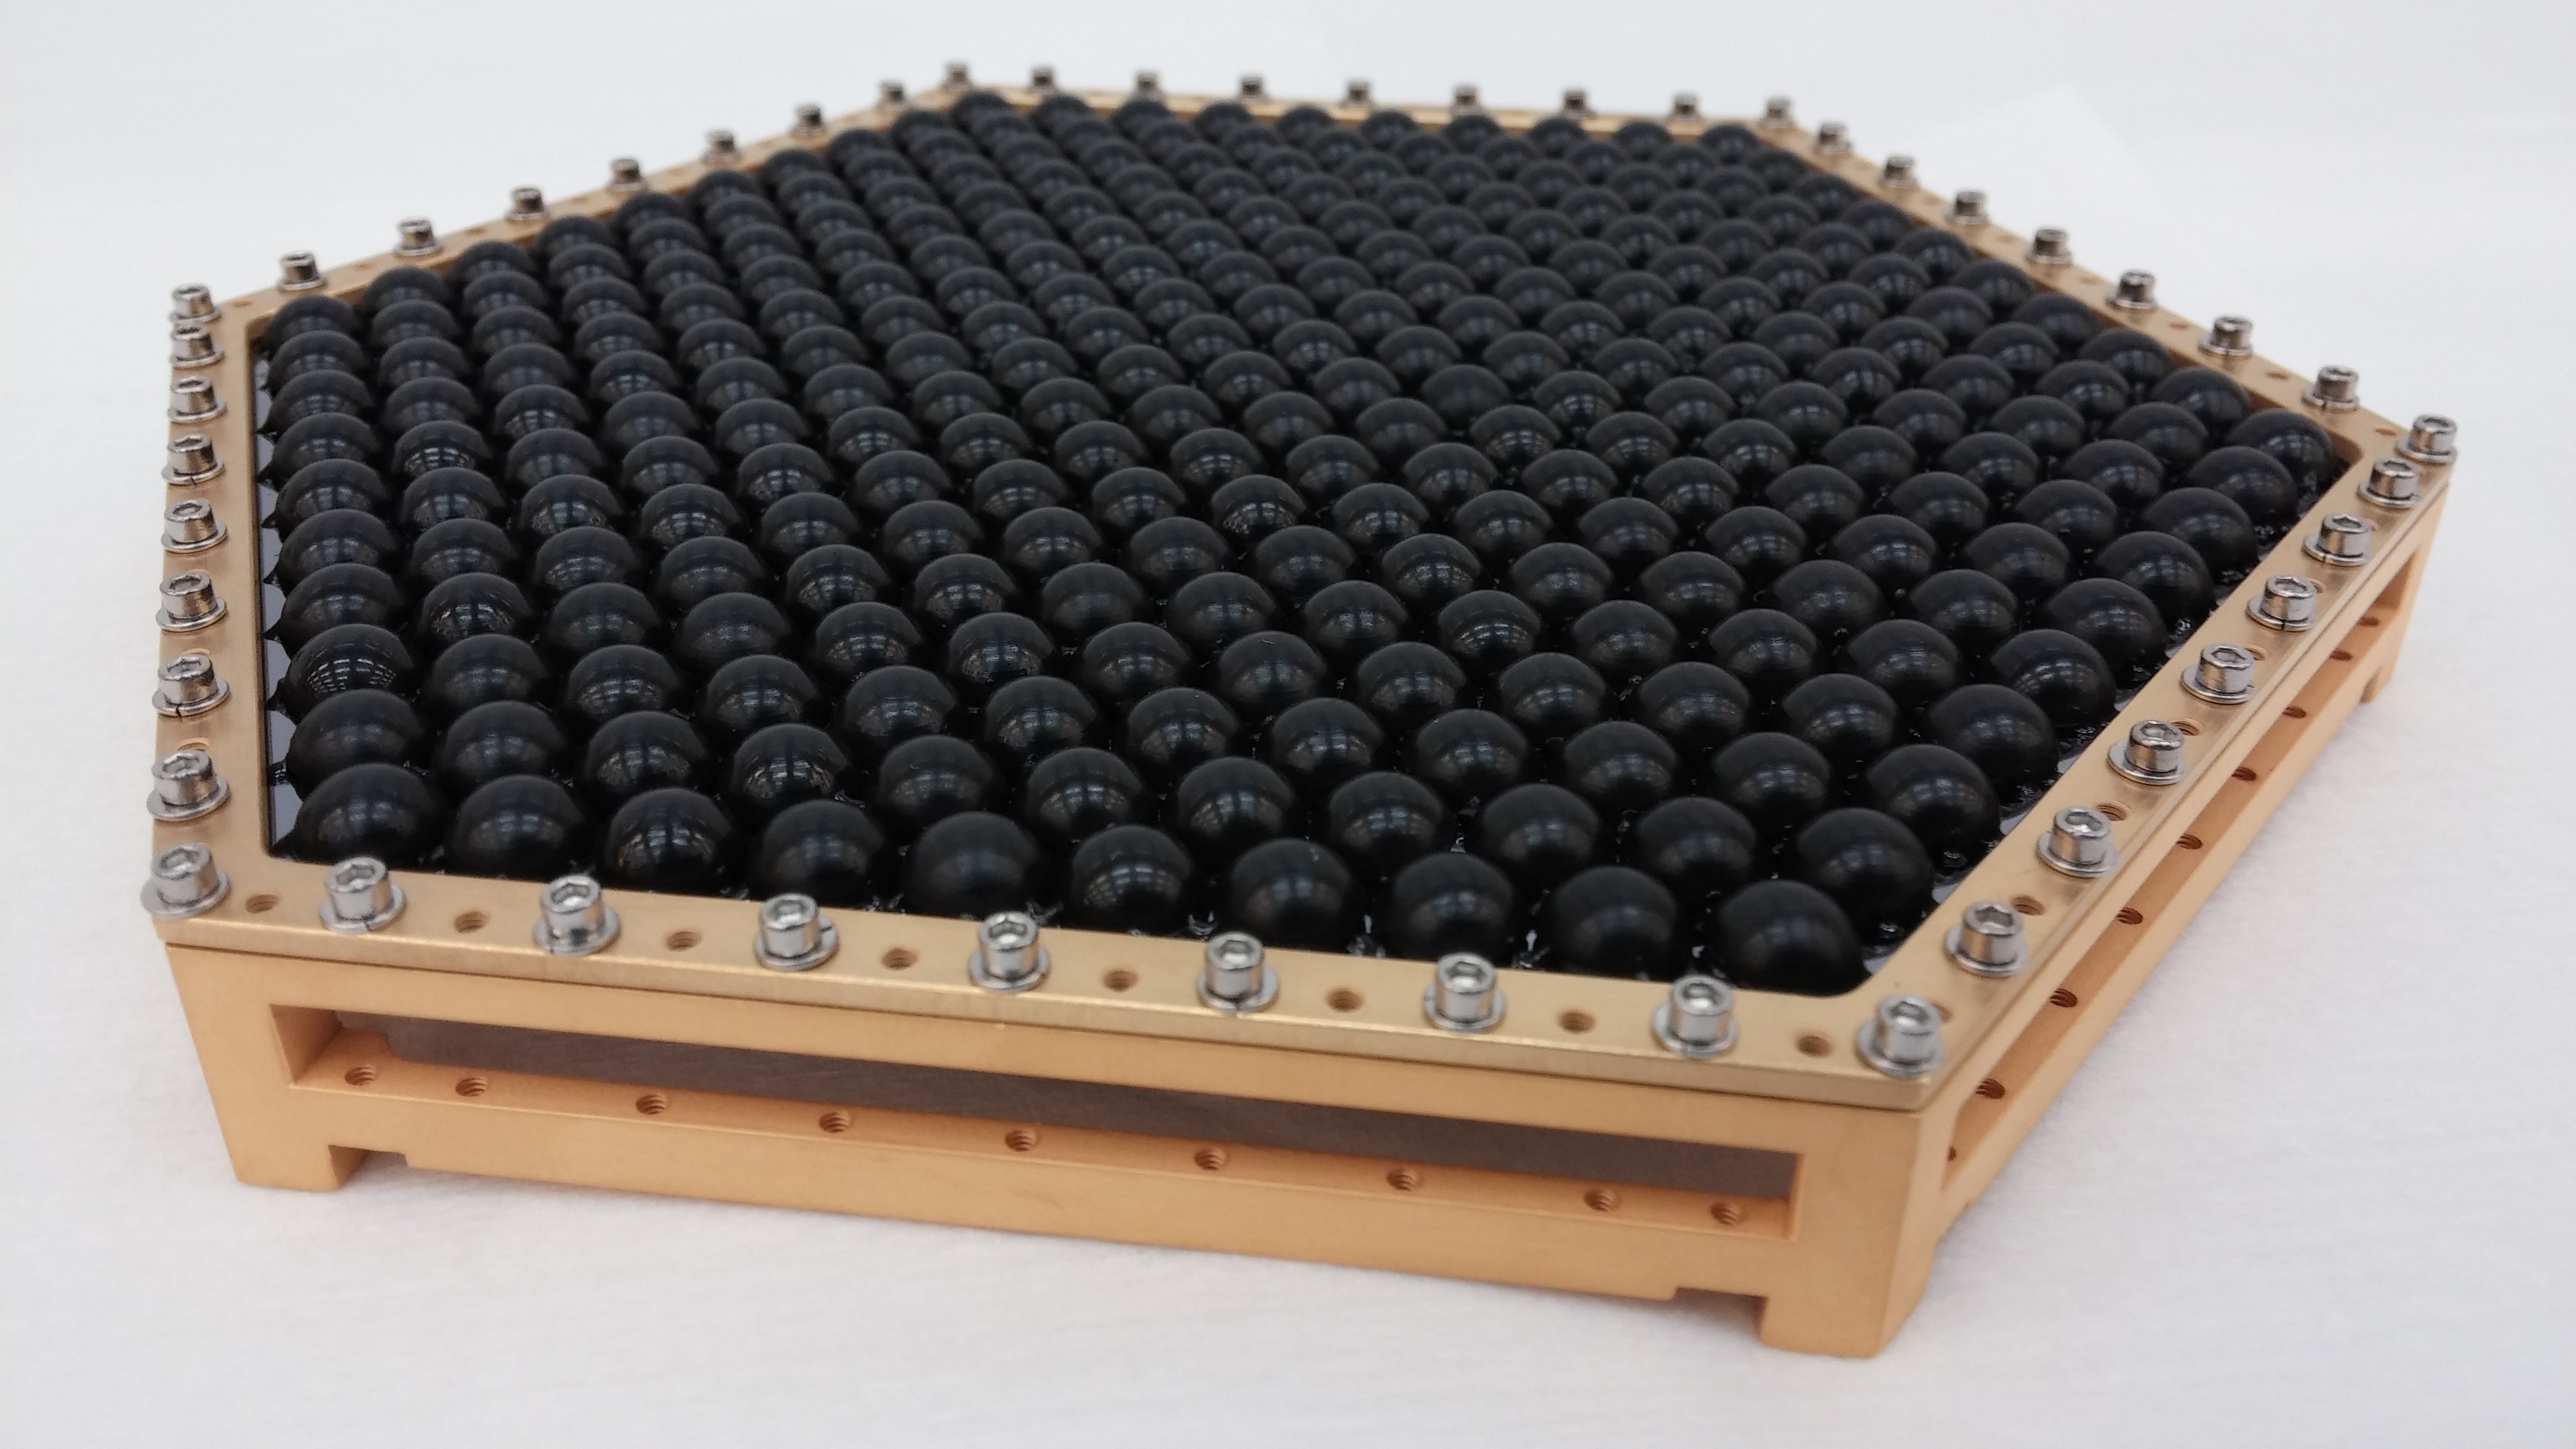
\includegraphics[width=0.48\linewidth, trim=0cm -1cm 0cm 0cm, clip]{InstrumentOverview/Figures/PB2_lenslets.jpg}}
    \hfill
    \subfloat[\label{fig:focal_plane_optics:c}]{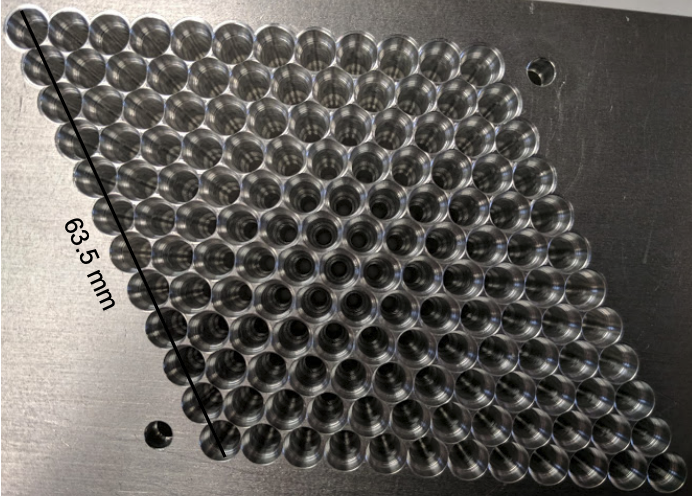
\includegraphics[width=0.48\linewidth, trim=0cm 0cm 0cm 0cm, clip]{InstrumentOverview/Figures/SO_horns.png}}
    \subfloat[\label{fig:focal_plane_optics:d}]{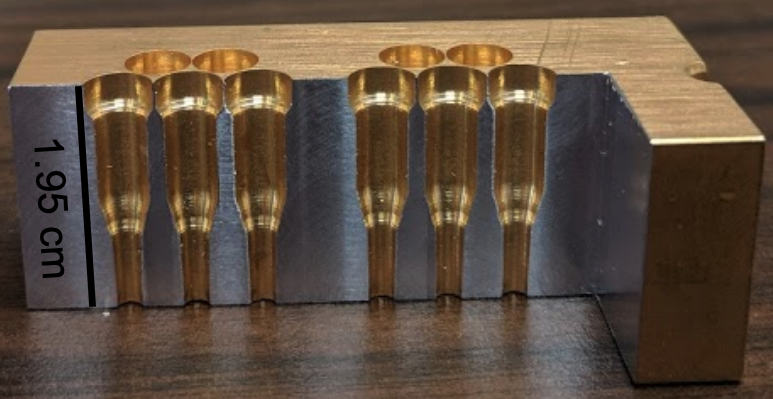
\includegraphics[width=0.48\linewidth, trim=0cm -2.9cm 0cm 0cm, clip]{InstrumentOverview/Figures/SO_horns_crossSection.png}}
    \caption[Simons Array and Simons Observatory focal plane optics]{SA and SO focal plane optics. (a) shows a PB-2a wafer, which has 271 dichroic detector pixels comprised of sinuous antennas which sense 90 and 150~GHz, and (b) shows the lenslet array that focuses light onto the antennas. In this photo, the lenslets are AR coated with two layers of Stycast, which is the lenslet technology used by PB-2a and PB-2b, but PB-2c and SO are researching alternative lenslet AR coating technologies. (c) and (d) show a prototype feedhorn array for 90/150~GHz pixels on SO. The spline profile optimizes for favorable beam properties while packing the pixels closely without optical crosstalk. Sinuous and lenselt photos courtesy of Aritoki Suzuki, and feedhorn photos courtesty of Sara Simon.}
    \label{fig:focal_plane_optics}
\end{figure}

The SA detector arrays are composed of seven \important{detector wafers}, each of which contains 271 detector pixels. The sensing element for the SA detector pixels is a planar sinuous antenna coupled to a hemispherical lenslet. The reimaging lenses focus the light onto the tip of the lenslet, which in turn re-focuses the light onto the antenna feed. The sinuous antenna is a fractal antenna whose logarithmically repeating pattern make sensitivie over a broad bandwidth. The high- and low-frequency cutoffs of the antenna are set by the minimum feature size and by the overall antenna size, respectively. After the incident radiation is collected by the antenna, a transmission line carries the light through on-chip bandpass filters, which separate the 90~and~150~GHz bands while rejecting out-of-band radiation. The band-pass-admitted radiation is then dissipated onto a thermistor whose output is amplified, digitized, and stored as raw data. To ensure efficient coupling to the sinuous antenna, the lenslets are manufactured as precise hemispheres, are offset from the sinuous antenna by a silicon spacing wafer, and are oversized to ensure adequate collimation.

The SO LF detector arrays use the same lenslet-coupled antenna technique that SA does, but its MF and UHF arrays instead employ feed horns coupled to planar, lithographed polarization-discriminating orthomode transducers. A feed horn is effectively an impedance-matched waveguide, designed to transform waves propagating in free space into wave-guide modes, which can then be routed, manipulated, and detected. Feed horns come in many different varieties, and perhaps the most common type have corrugations along its walls to prevent substrate modes that can in turn induce a side-lobe response. While corrugations are a tried and true technique to obtain a Gaussian, symmetric pixel response, they are not space efficient and therefore give rise to a substantial fraction of the focal plane area being optically inactive. To combat this issue, SO (building the work of Advanced ACT) uses smooth-walled feed horns with spline-profiled shapes to optimize over several performance metrics, including coupling to the telescope optics, cross polarization, and beam shape. Without corrugations, the array of feed horns can be very dense, with only hundreds of microns separating adjacent detector pixels. This setup in turn increases the detector count per telescope, which improves the sensitivity of the experiment.

%%%%%%%%%%%%%%%%%%%%%%%%%%%%%%%%
%%%%%%%%%%%%%%%%%%%%%%%%%%%%%%%%

\subsection{Telescope to focal plane coupling}
\label{sec:beam_coupling}

Given a high-level overview of the SA and SO pixel architectures, we now move to quantify the coupling between the focal plane and the telescope, which is central to many of the sensitivity calculations in following chapters. Assuming a diffraction-limited optical system, the magnification of the optics tube is quantified by the \important{F-number} (also sometimes called the ``focal ratio'') at the focal plane
\begin{equation}
    F = \frac{D_{\mathrm{apert}}}{f} \, ,
    \label{eq:fnumber}
\end{equation}
where $D_{\mathrm{apert}}$ is the diameter of the aperture stop (or, for the SA telescope and SO LAT, the Lyot stop) and $f$ is the focal length of the focal plane image. The F-number quantifies the magnification of the optical system: given a fixed aperture size, a larger/smaller F-number leads to a smaller/larger focal plane size or equivalently a smaller/larger magnification.

\begin{figure}
    \centering
    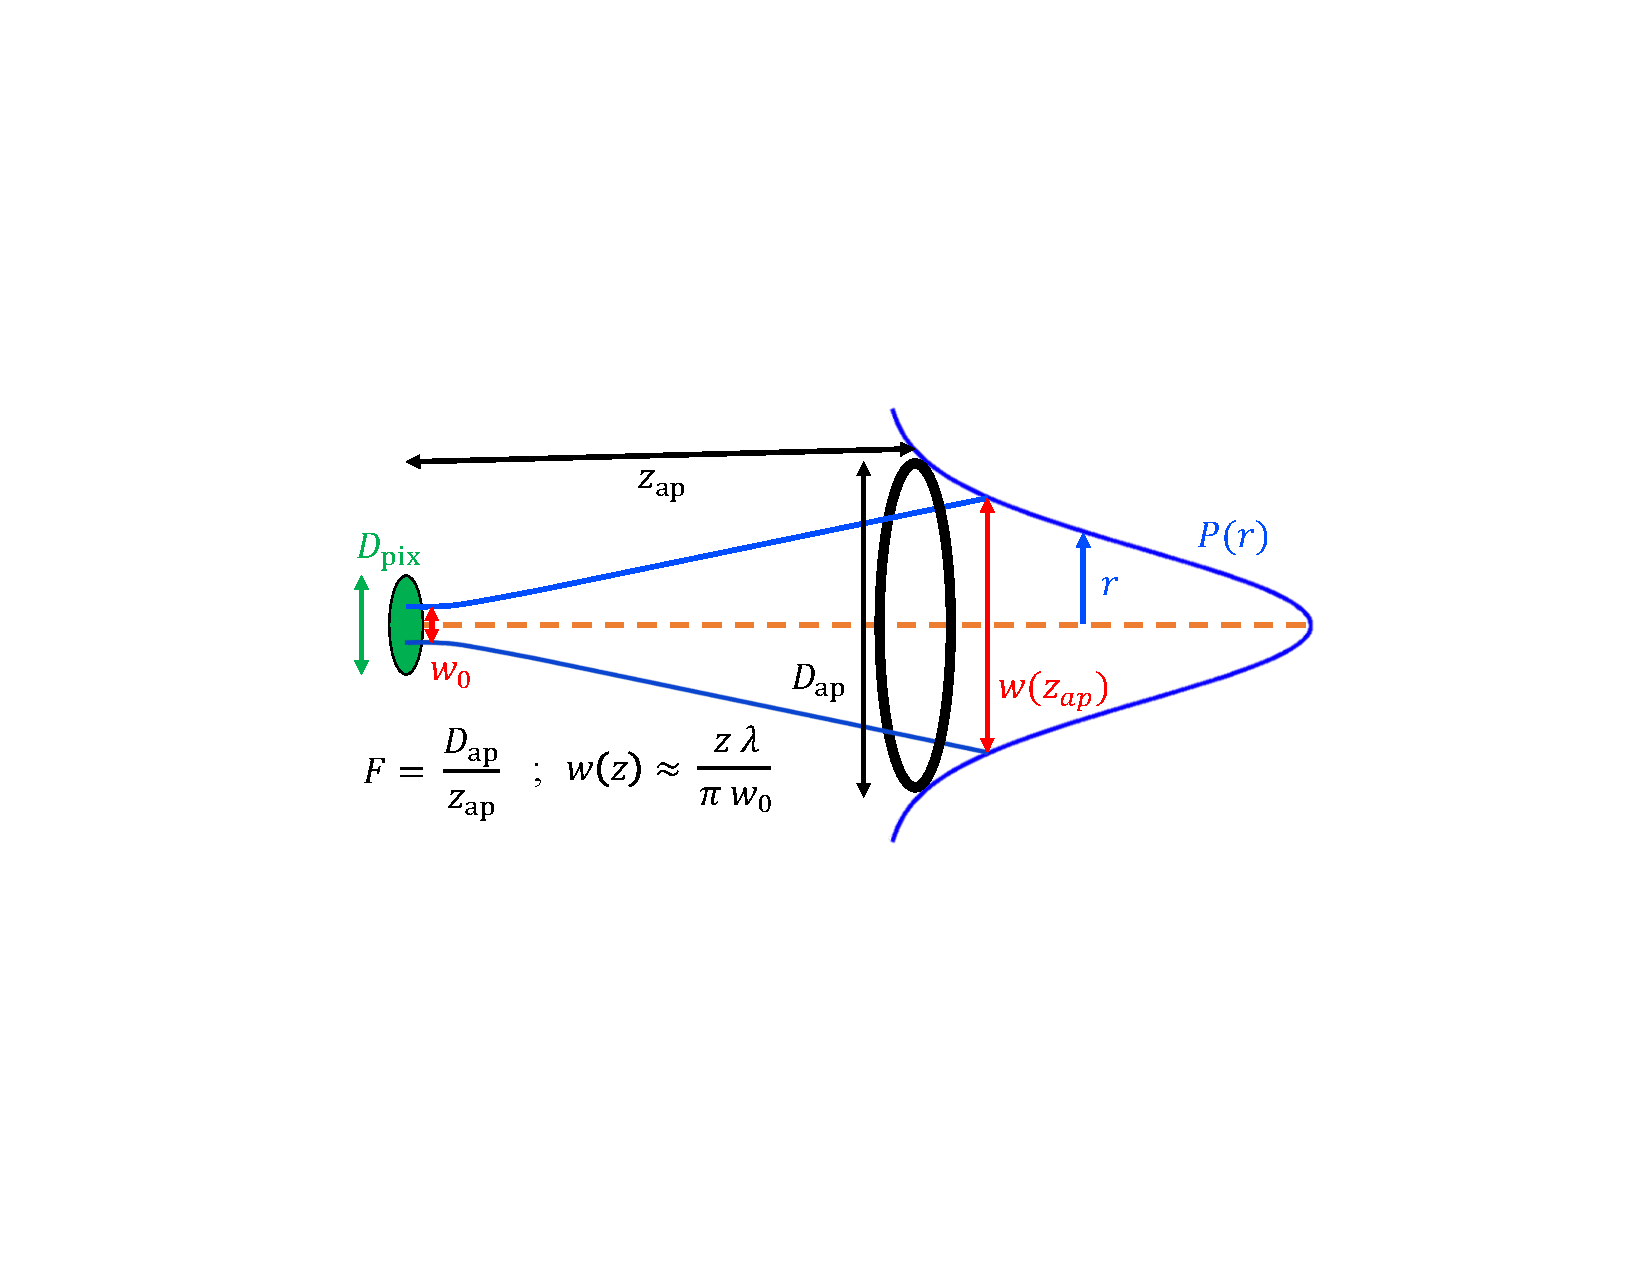
\includegraphics[width=\linewidth, trim=5cm 7cm 5cm 7cm, clip]{InstrumentOverview/Figures/beam_coupling_efficiency.pdf}
    \caption{A schematic of how the green detector pixel with diameter $D_{\mathrm{pix}}$ might illuminate the aperture stop of diameter $D_{\mathrm{ap}}$ and distance $z_{\mathrm{ap}}$ from the focal plane. The size of the beam at the aperture $w(z)$ is inversely proportional to its beam waist $w_{0}$, and the approximation applies in the \important{Rayleigh limit} where $z \gg w_{0}$.}
    \label{fig:beam_coupling_efficiency}
\end{figure}

As long as the pixels are large compared to the wavelength, they will induce minimal diffractive ringing, and therefore their \important{beam} (or equivalently, their response as a function of opening angle and/or x/y/z position) is well-approximated by a Gaussian function. In particular, detector's far-field response is given as
\begin{equation}
    B_{\mathrm{pix}}(\theta, \lambda) = \exp \left( \frac{-\theta^{2}}{2 \theta_{\mathrm{pix}}^{2}} \right) \, ,
    \label{eq:detector_pixel_beam}
\end{equation}
$\theta$ is the ray angle with respect to zenith and where
\begin{equation}
    \theta_{\mathrm{pix}} = \frac{\lambda}{\pi w_{0}} \, .
    \label{eq:pixel_beam_divergence}
\end{equation}
Here, the angular width of the pixel beam is inversely proportional to its \important{beam waist} $w_{0}$, which in turn can be related to the pixel diameter $D_{\mathrm{pix}}$ under the assumption of diffraction-limited optics
\begin{equation}
    w_{0} = \frac{D_{\mathrm{pix}}}{w_{\mathrm{f}}} \, .
\end{equation}
The most important result of this diffraction-limited formalism is that larger/smaller pixels produce a tighter/wider beam, and this in turn impacts how the detector pixel couples to the telescope.

There are two useful ways to conceptualize the relationship between the telescope and focal plane optics. The first way is to think in the forward-time sense, which is to imagine photons propagating from the sky to the detectors. In this paradigm, the image formed by the telescope becomes smaller with larger F-number (larger magnification), which in turn favors smaller pixels. The second and equally valid way is to think in the \important{reverse-time sense}, which is to imagine photons propagating form the detectors to the sky. In this paradigm, a larger F-number corresponds to a wider aperture, which in turn favors a wider pixel beam. While these two paradigms are equivalent, it will be most convenient to calculate telescope-pixel coupling efficiency from the pixel's perspective, in the reverse-time sense.

From the perspective of the detector pixel, the opening half angle of the aperture stop is
\begin{equation}
    \theta_{\mathrm{f}} = \arctan \left( \frac{1}{2 F} \right) \approx \frac{1}{2 F}\, ,
    \label{eq:stop_angle}
\end{equation}
where the approximation applies in the \important{paraxial limit}, or the small-angle regime. Given this angle, the coupling between the telescope and the detector pixel's beam is often called the \textit{beam coupling efficiency}
\begin{equation}
    \eta_{\mathrm{apert}} = \frac{\int_{0}^{{\theta_{\mathrm{f}}}} B_{\mathrm{pix}}(\theta, \lambda) \dd \theta}{\int_{0}^{{\pi / 2}} B_{\mathrm{pix}}(\theta, \lambda) \dd \theta} = 1 - \exp \left[ -\frac{\theta_{\mathrm{f}}^{2}}{2 \theta_{\mathrm{pix}}^{2}} \right] \approx 1 - \exp \left[ -\frac{1}{2} \left( \frac{\pi D_{\mathrm{pix}}}{w_{\mathrm{f}} F \lambda} \right)^{2} \right] \, ,
    \label{eq:beam_coupling_efficiency}
\end{equation}
where again the second equivalent relies on the paraxial approximation. Note that this beam-spill treatment only applies in the diffraction-limited paradigm, which has a constant throughput of $A \Omega = \lambda^{2}$. In other words, making the pixel bigger does not change the amount of light it can collect, but only the size of its far-field illumination.

\begin{figure}[!t]
    \centering
    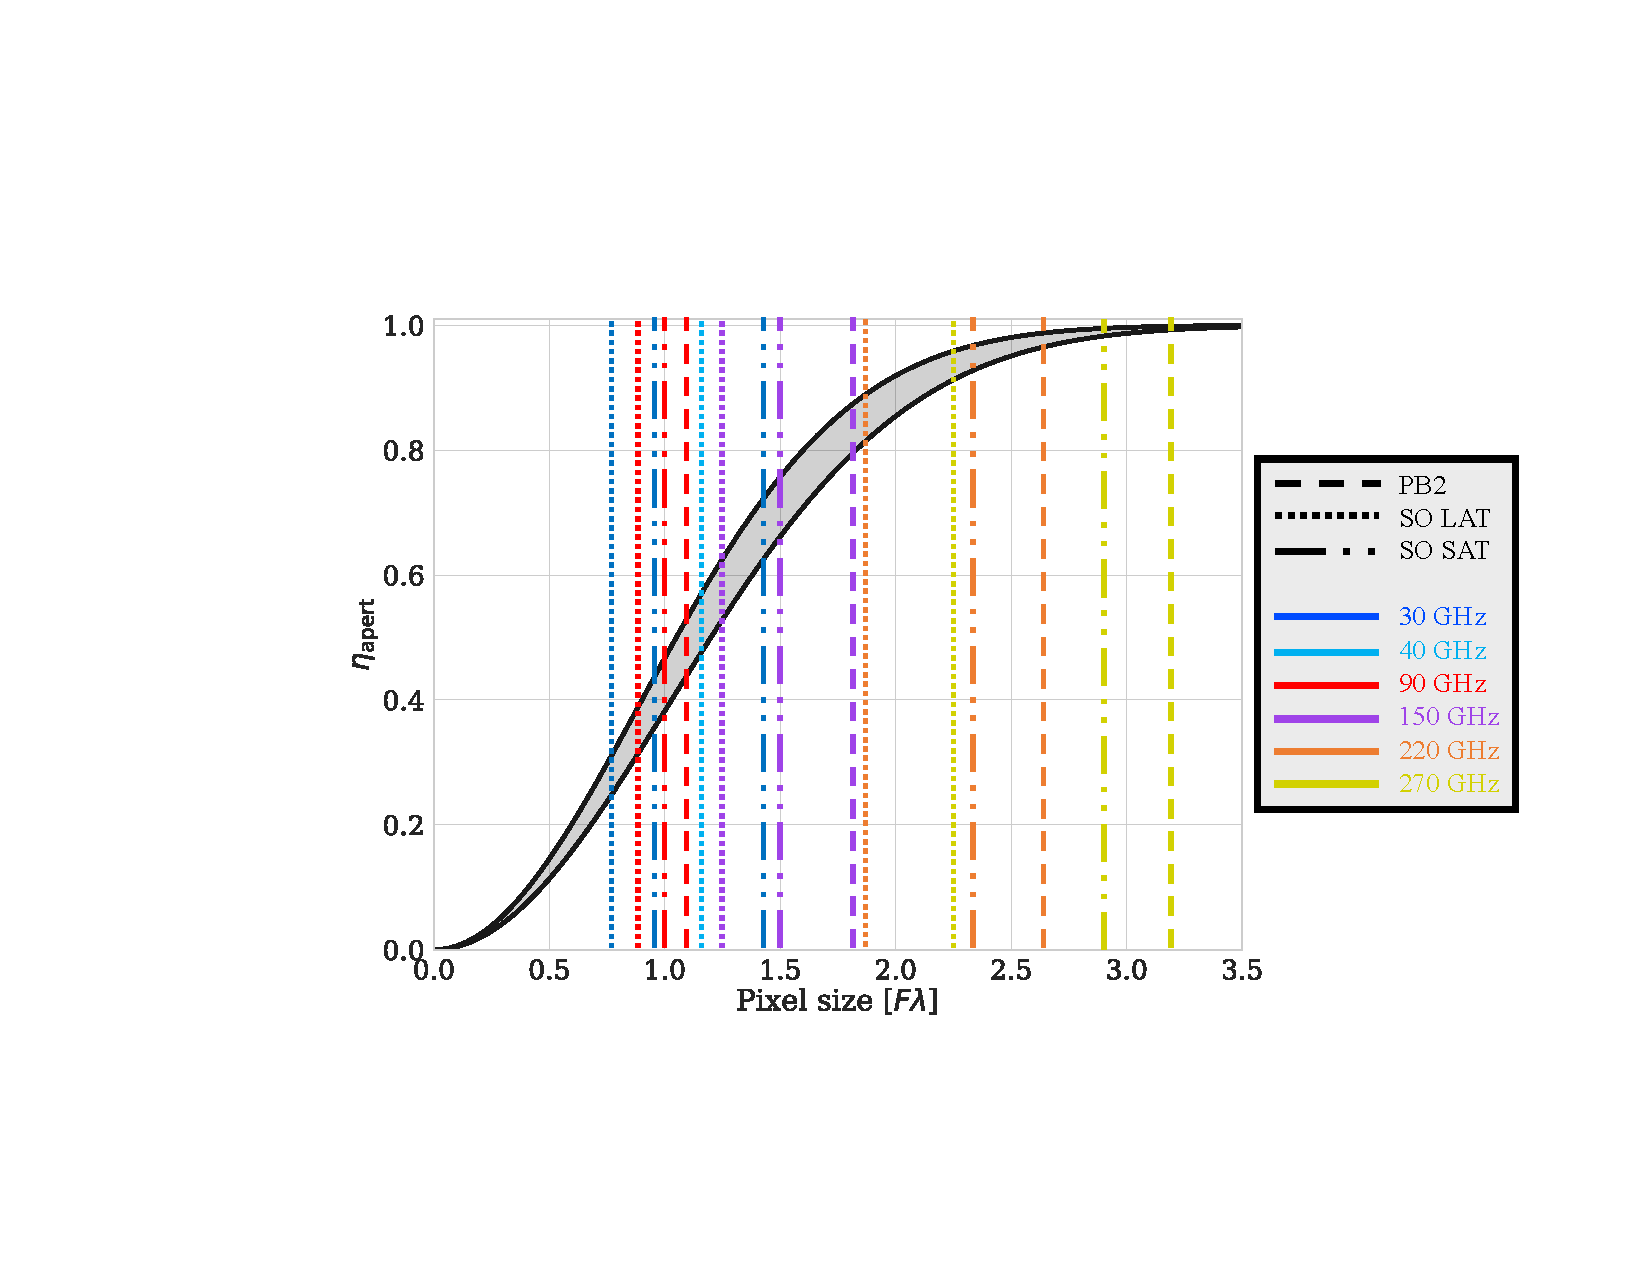
\includegraphics[width=\linewidth, trim=5cm 4cm 1cm 5cm, clip]{InstrumentOverview/Figures/aperture_eff_pix_sizes.pdf}
    \begin{tabular}{m{3.5cm}|m{3.5cm}|m{2cm}|m{3.5cm}|m{0.7cm}}
         Pixel & Coupling & $D_{\mathrm{pix}}$ [mm] & $D_{\mathrm{pix}} / F \lambda$ & $\eta_{\mathrm{spill}}$ \\
         \hline
         \hline
         SA 90/150~GHz & Lenslet + Sinuous & 6.8 & \shortstack{90~GHz: 1.1 \\ 150~GHz: 1.8} & \shortstack{0.54 \\ 0.85} \\
         \hline
         SA 220/270~GHz & Lenslet + Sinuous & 6.8 & \shortstack{220~GHz: 2.6 \\ 270~GHz: 3.2} & \shortstack{0.98 \\ 0.99} \\
         \hline
         SO LF & Lenslet + Sinuous & 18.3 & \shortstack{30~GHz LAT: 0.8 \\ 30~GHz SAT: 1.0 \\ 40~GHz LAT: 1.1 \\ 40~GHz SAT: 1.5} & \shortstack{0.25 \\ 0.37 \\ 0.48 \\ 0.65}\\
         \hline
         SO MF & Feed horn & 5.3 & \shortstack{90~GHz LAT: 0.8 \\ 90~GHz SAT: 1.0 \\ 150~GHz LAT: 1.2 \\ 150~GHz SAT: 1.5} & \shortstack{0.25 \\ 0.37 \\ 0.51 \\ 0.71} \\
         \hline
         SO UHF & Feed horn & 5.3 & \shortstack{220~GHz LAT: 1.8 \\ 220~GHz SAT: 2.3 \\ 270~GHz LAT: 2.2 \\ 270~GHz SAT: 2.9} & \shortstack{0.79 \\ 0.92 \\ 0.90 \\ 0.97} \\
         \hline
    \end{tabular}
    \caption{Beam coupling efficiencies for SA and SO detectors. The top panel shows the shows the loation of the pixel sizes in units of $F \lambda$ along the $\eta_{\mathrm{apert}}$ curve, and the shaded region represents $2.8 \geq w_{\mathrm{f}} \geq 3.2$. There is a clear clustering of pixel sizes in the area of 1.0~$F \lambda$, which is a natural optimum that we discuss in great detail in Chapter~\ref{ch:white_noise_correlations}.}
    \label{fig:beam_coupling_eff_pixel_sizes}
\end{figure}



As evidenced by the beam coupling efficiencies in Table~\ref{tab:beam_coupling_efficiencies}, the SA and SO detector pixels are substantially illuminating the stop. While this degrades per-detector sensitivity, it allows more detectors to be packed onto the focal plane, improving overall instrument performance. In this paradigm, it is critically important for the aperture stop to be as cold as possible to limit the parasitic loading on the detectors. 

%%%%%%%%%%%%%%%%%%%%%%%%%%%%%%%%
%%%%%%%%%%%%%%%%%%%%%%%%%%%%%%%%

\subsection{Anti-reflection coatings}
\label{sec:instrument_overview_ar_coatings}

SA and use alumina and silicon refracting optics, which have a large index of refraction ($n_{\mathrm{alumina}} \approx 3.1$, $n_{\mathrm{silicon}} \approx 3.4$) compared to that of vacuum $n = 1$. Therefore, without anti-reflection (AR) coatings, a bare vacuum-optic interface, will have a reflectivity of $R = [(n - 1) / (n + 1)]^{2} \sim 30$\% at normal incidence and even worse at oblique angles. Given that each lens has two surfaces and that there are three lenses per optics tube, the transmittivity of the receiver without any anti-reflection (AR) coatings would be $T = (1 - r)^{6} = 15$\%. In addition, such large reflectivities encourage multiple reflections within the cryostat that can great near-field images that can show up as \textit{ghosts} in the resulting sky image. Therefore, AR coatings play a critical role in the optical performance of the receiver. AR coatings are discussed in greater detail in Section~blah.

\begin{figure}[!t]
    \centering
    \subfloat[\label{fig:cmb_instrument_ar_coatings:a}]{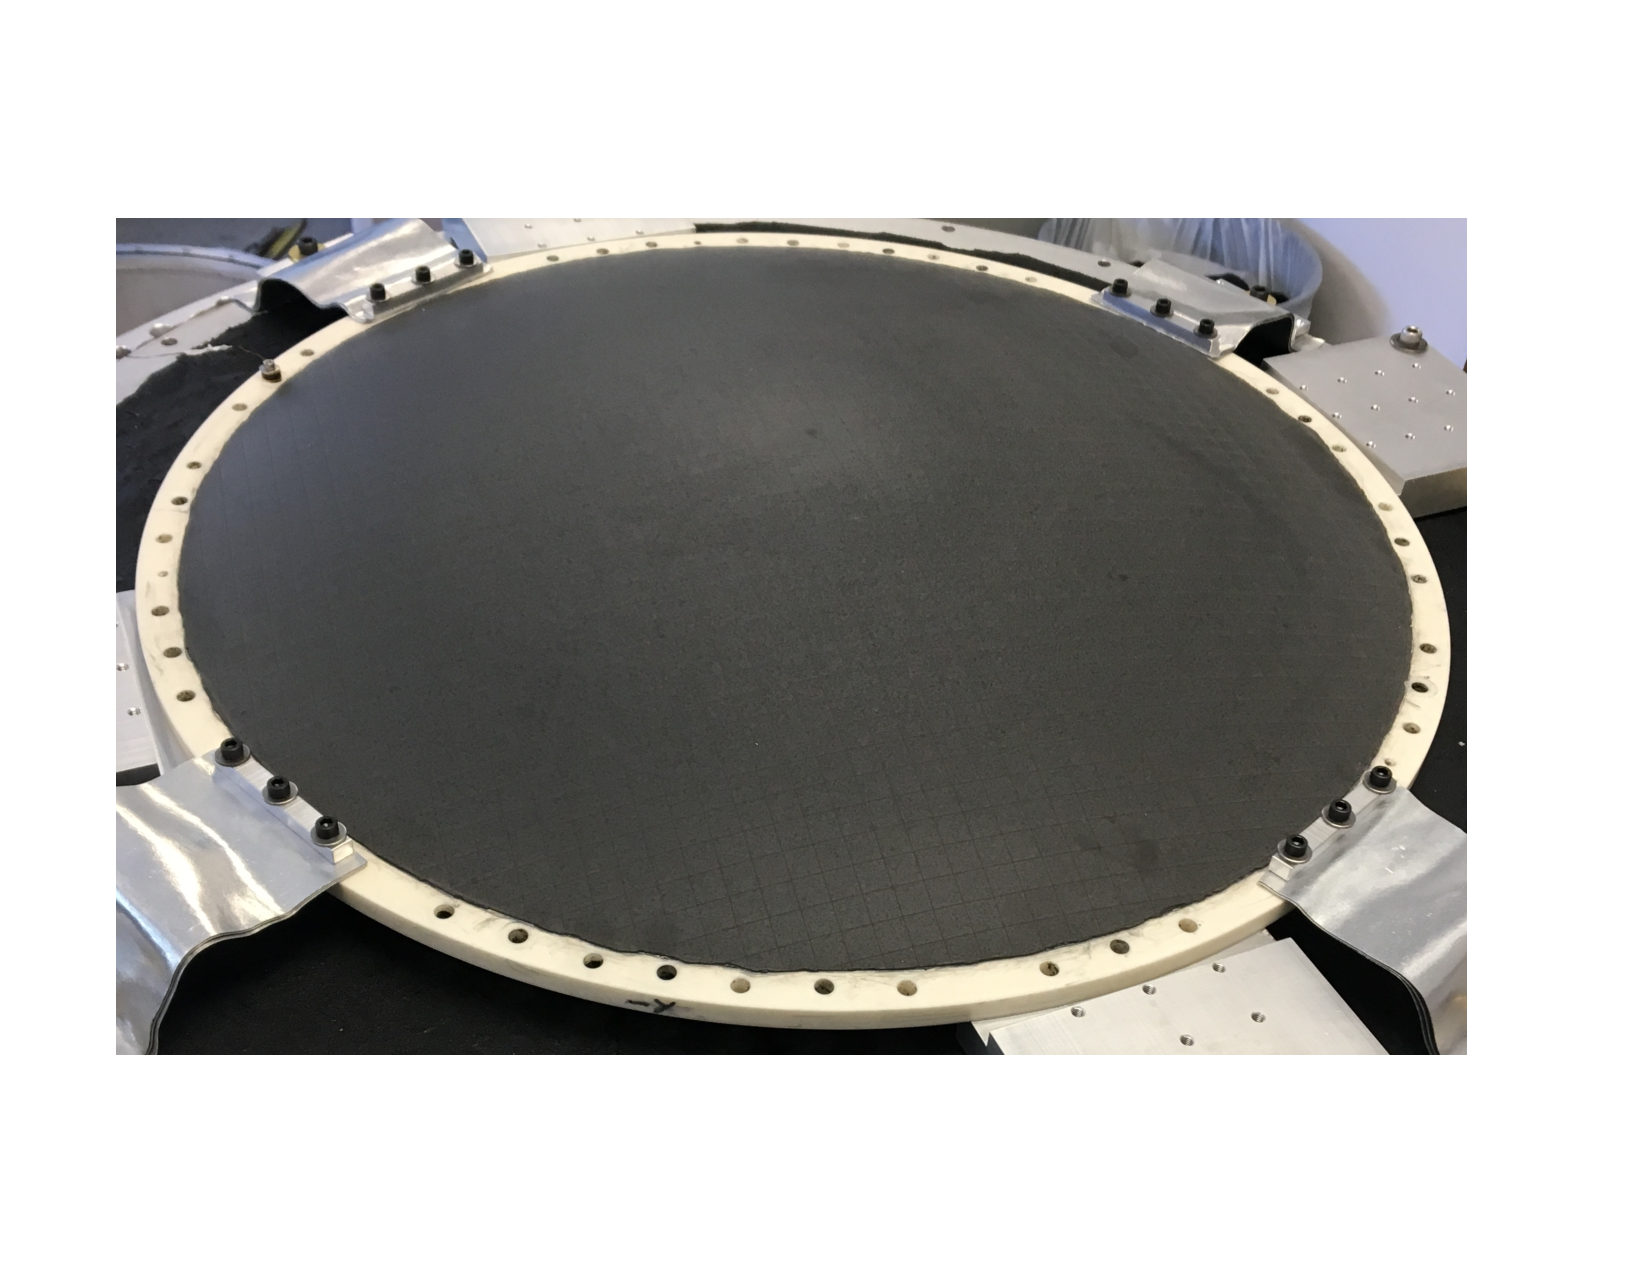
\includegraphics[width=0.48\linewidth, trim=2cm 4cm 2cm 4cm, clip]{InstrumentOverview/Figures/epoxy_ar_coating_example.pdf}}
    \subfloat[\label{fig:cmb_instrument_ar_coatings:b}]{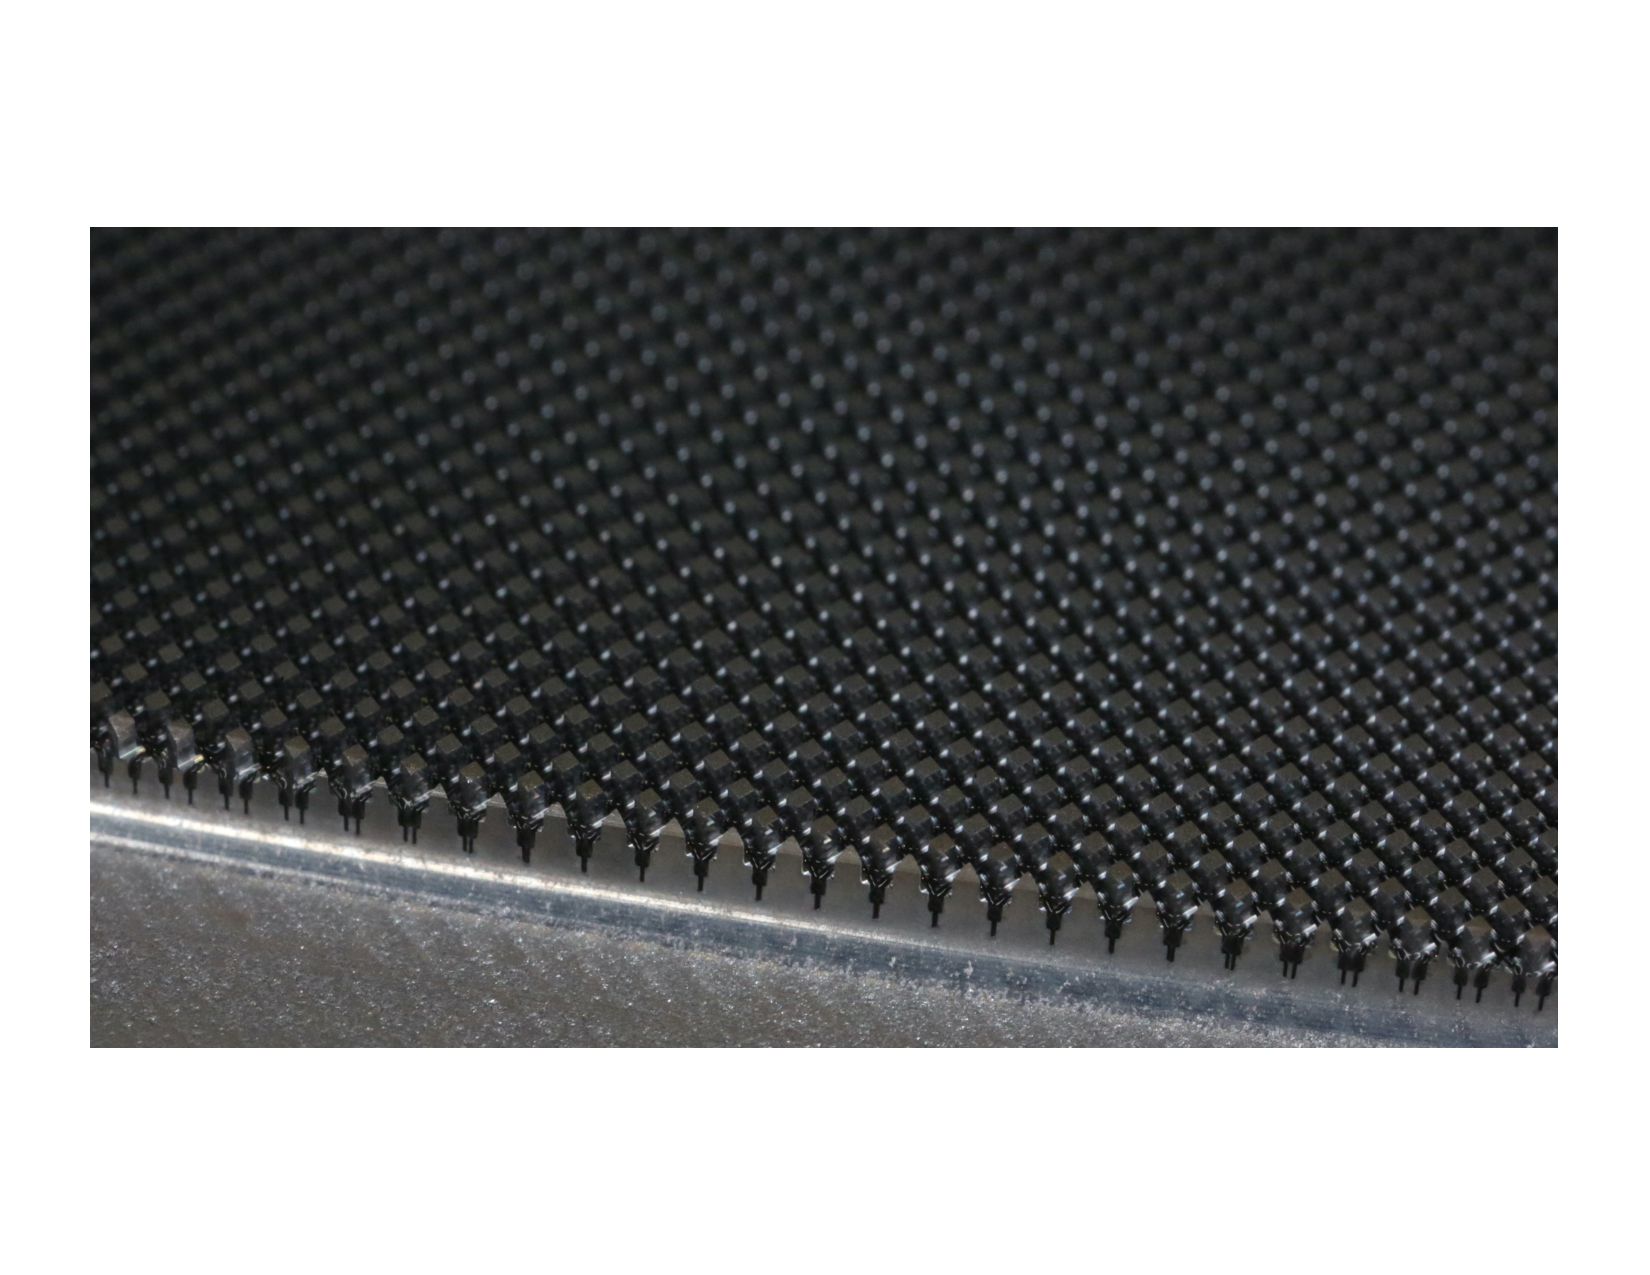
\includegraphics[width=0.48\linewidth, trim=2cm 4cm 2cm 4cm, clip]{InstrumentOverview/Figures/metamaterial_ar_coating_example.pdf}}
    \caption{AR coating technologies used within SA and SO. (a) shows the PB-2b field lens coated with two layers of epoxy mounted in a cryostat at LBNL right before thermal testing. The dicing lines are for strain relief and are cut by a UV laser, and the diameter of the part is 500~mm. (b) shows an SO MF silicon lens with three layers of metamaterial AR. The pitch between ``pillars'' is 0.4~mm. The silicon photo is courtesy of Joey Golec.}
    \label{fig:cmb_instrument_ar_coatings}
\end{figure}

SA's alumina/silicon AR coatings are composed of several technologies that have matured during the course of the project. All coatings are dicrhoic and comprise two distinct layers with optimal index and optimal thickness. In PB-2a, the curved sides of the lenses are coated with two layers of Stycast epoxy, which is molded onto the surface during the epoxy cure and milled to thickness after the mold is removed. The flat sides of the lenses are coated with a bottom layer of plasma-sprayed Mullite and a top layer of an expanded polyimide foam glued using melted low-density polyethylene. The former technology was developed at Berkeley in California, while the latter was developed at the KEK high-energy laboratory in Japan. PB-2 and PB-2c, on the other hand use plasma-sprayed alumina loaded with various fillers to adjust the layer's index. The layers are applied directly onto the lens surface with a finely tuned thickness, and the density is controlled via tuning of plasma-spay parameters, which in turn controls the layer density. Each of these technologies have their own advantages and disadvantages, but all of them attain a reflectivity of $\sim$~1\%, amounting to a total lens throughput of $\sim$~90\%. Given the huge importance of AR coatings in the receiver, the UC Berkeley group invests substantial resources into the development of higher-throughput, scalable, cost-effective AR coatings both for SA and for future experiments. This has led to substantial advancements in the technology, which we discuss in further detail in Section~blah.

SO's on the other hand uses \important{metamaterial} AR coatings for their alumina and silicon optics. This technique involves cutting sub-wavelength structures into the optic's surface whose geometry allows silicon/alumina and vacuum to combine to give an effective dielectric constant. This method has several advantages over the more ``traditional'' approach of adding materials to the surface. First, there are no concerns about cryogenic delamination, because there is no CTE mismatch between AR materials and the base lens materials. Second, the dielectric constant is (in theory) fully tunable via simply adjusting the sub-wavelength structure geometry. This tuning mechanism is in contrast to using plastics or epoxies, for example, which require a precise material composition to achieve the desired index that is often not easily tuned. Third, there is a smaller penalty for adding more layers, which is also driven by the lack of CTE mismatch issues. Therefore SO cuts three AR layers for their two-color instruments, which provides $\sim$~0.1\% in-band reflection, as opposed to two-layer coating which only achieves $\sim$~1\%. Not until recently have metamaterials on alumina been demonstrated, and therefore SO will be the first experiment to field sub-wavelength structures on ceramics.

%%%%%%%%%%%%%%%%%%%%%%%%%%%%%%%%
%%%%%%%%%%%%%%%%%%%%%%%%%%%%%%%%
%%%%%%%%%%%%%%%%%%%%%%%%%%%%%%%%

\section{Thermal Design}
\label{sec:optics_thermal_design}

In addition to providing a high-fidelity image of the sky onto the focal plane, the receiver the receiver optics need to reject huge amounts of infrared (IR) radiation in order to cool the detectors to sub-Kelvin temperatures. While the details of the SA and SO thermal filtering schemes differ in several ways, in this section we focus our discussion on that of SA, which will highlight the key principles of IR rejection while providing the necessary background information for SA thremal discussions in following chapters. 

As noted, the SA receiver has a 0.5~m diameter window and that the ambient temperature at the site is, on average, $\approx$~273~K, the radiative load on the cryostat is $\sim$~300~W. The sub-K refrigerator at a 0.3~K base temperature, on the other hand, has only $\sim$~5~$\mathrm{\mu W}$ of cooling power. Therefore, the receiver \important{optical stack}, which consists of not only its lenses but also several thermal filters, must reject power at one part $\sim 10^{8}$ while also being transparent to CMB photons at $\sim$~100~GHz.

\begin{figure}[!t]
    \centering
    \subfloat[\label{fig:pb2_filters:a}]{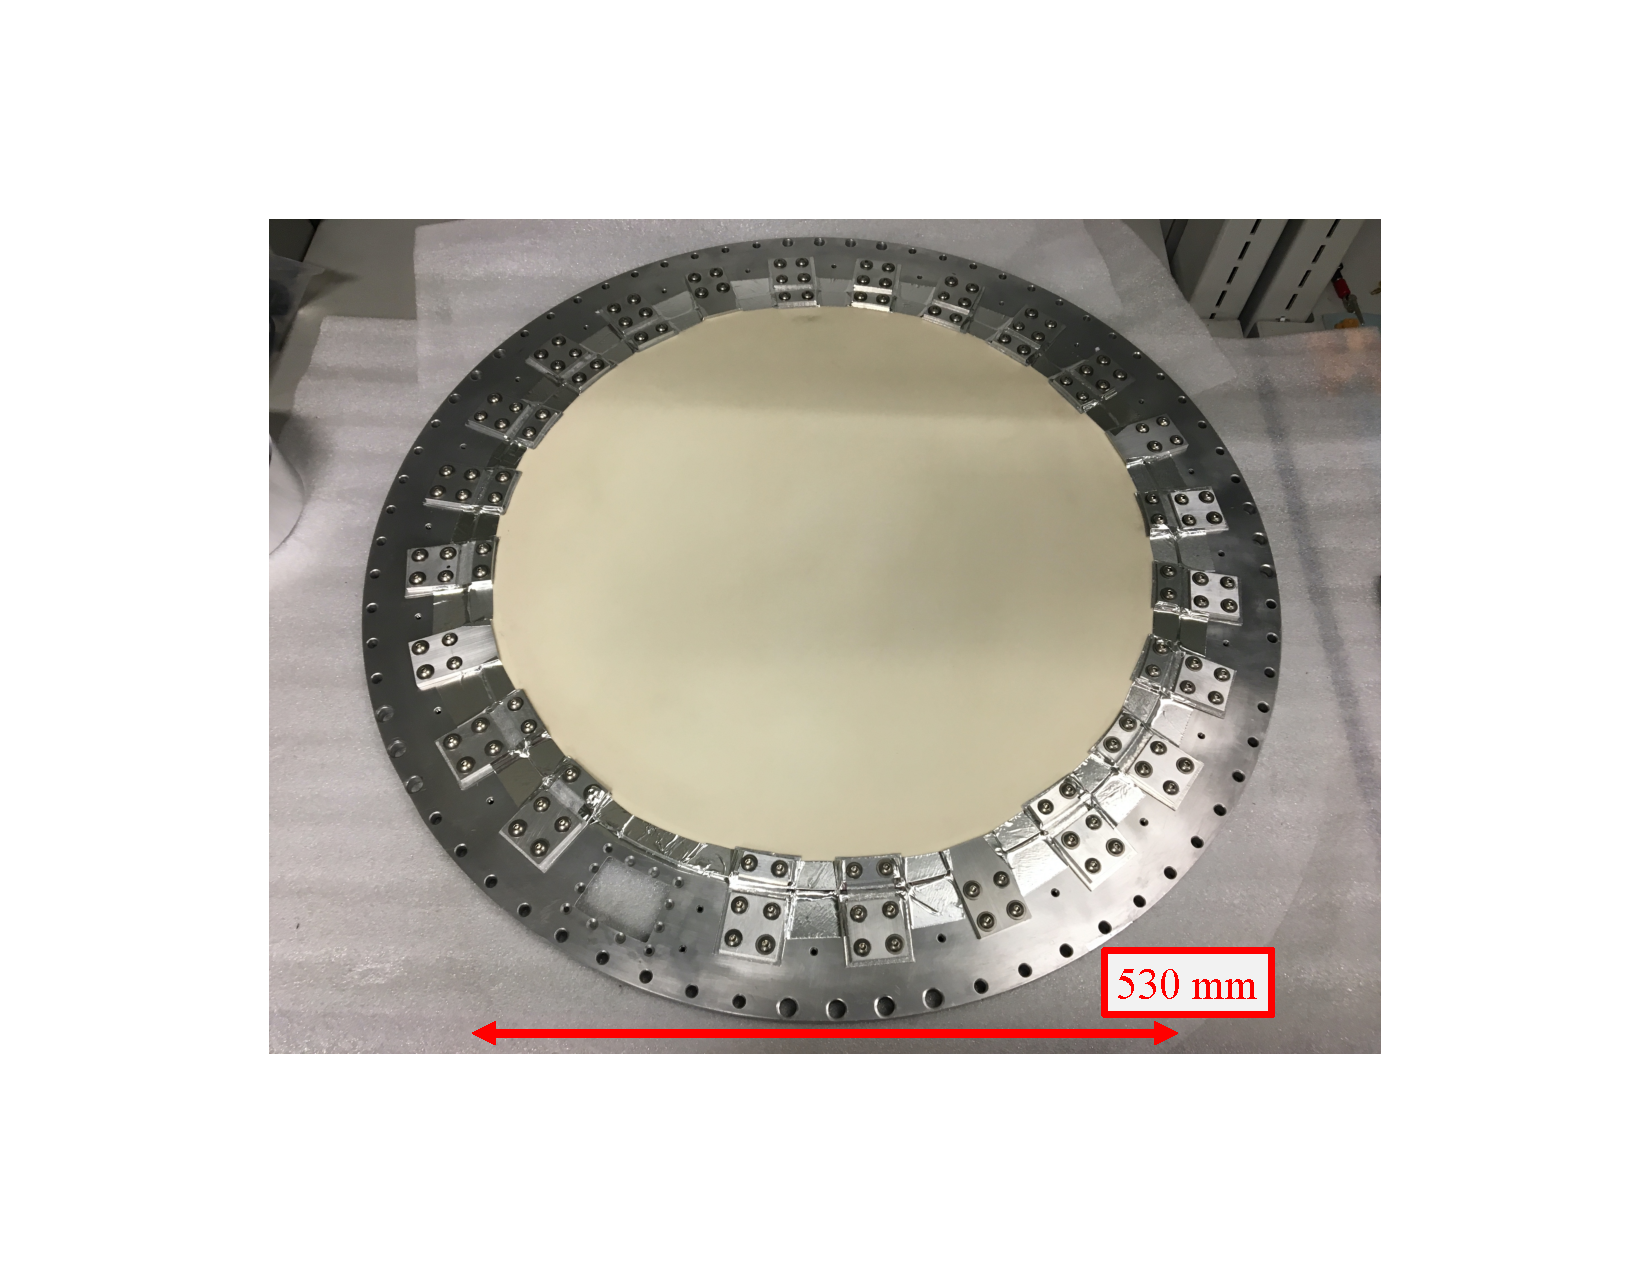
\includegraphics[width=0.48\linewidth, trim=5.5cm 3.5cm 5.5cm 3.5cm, clip]{InstrumentOverview/Figures/IRF_photo.pdf}}
    \subfloat[\label{fig:pb2_filters:b}]{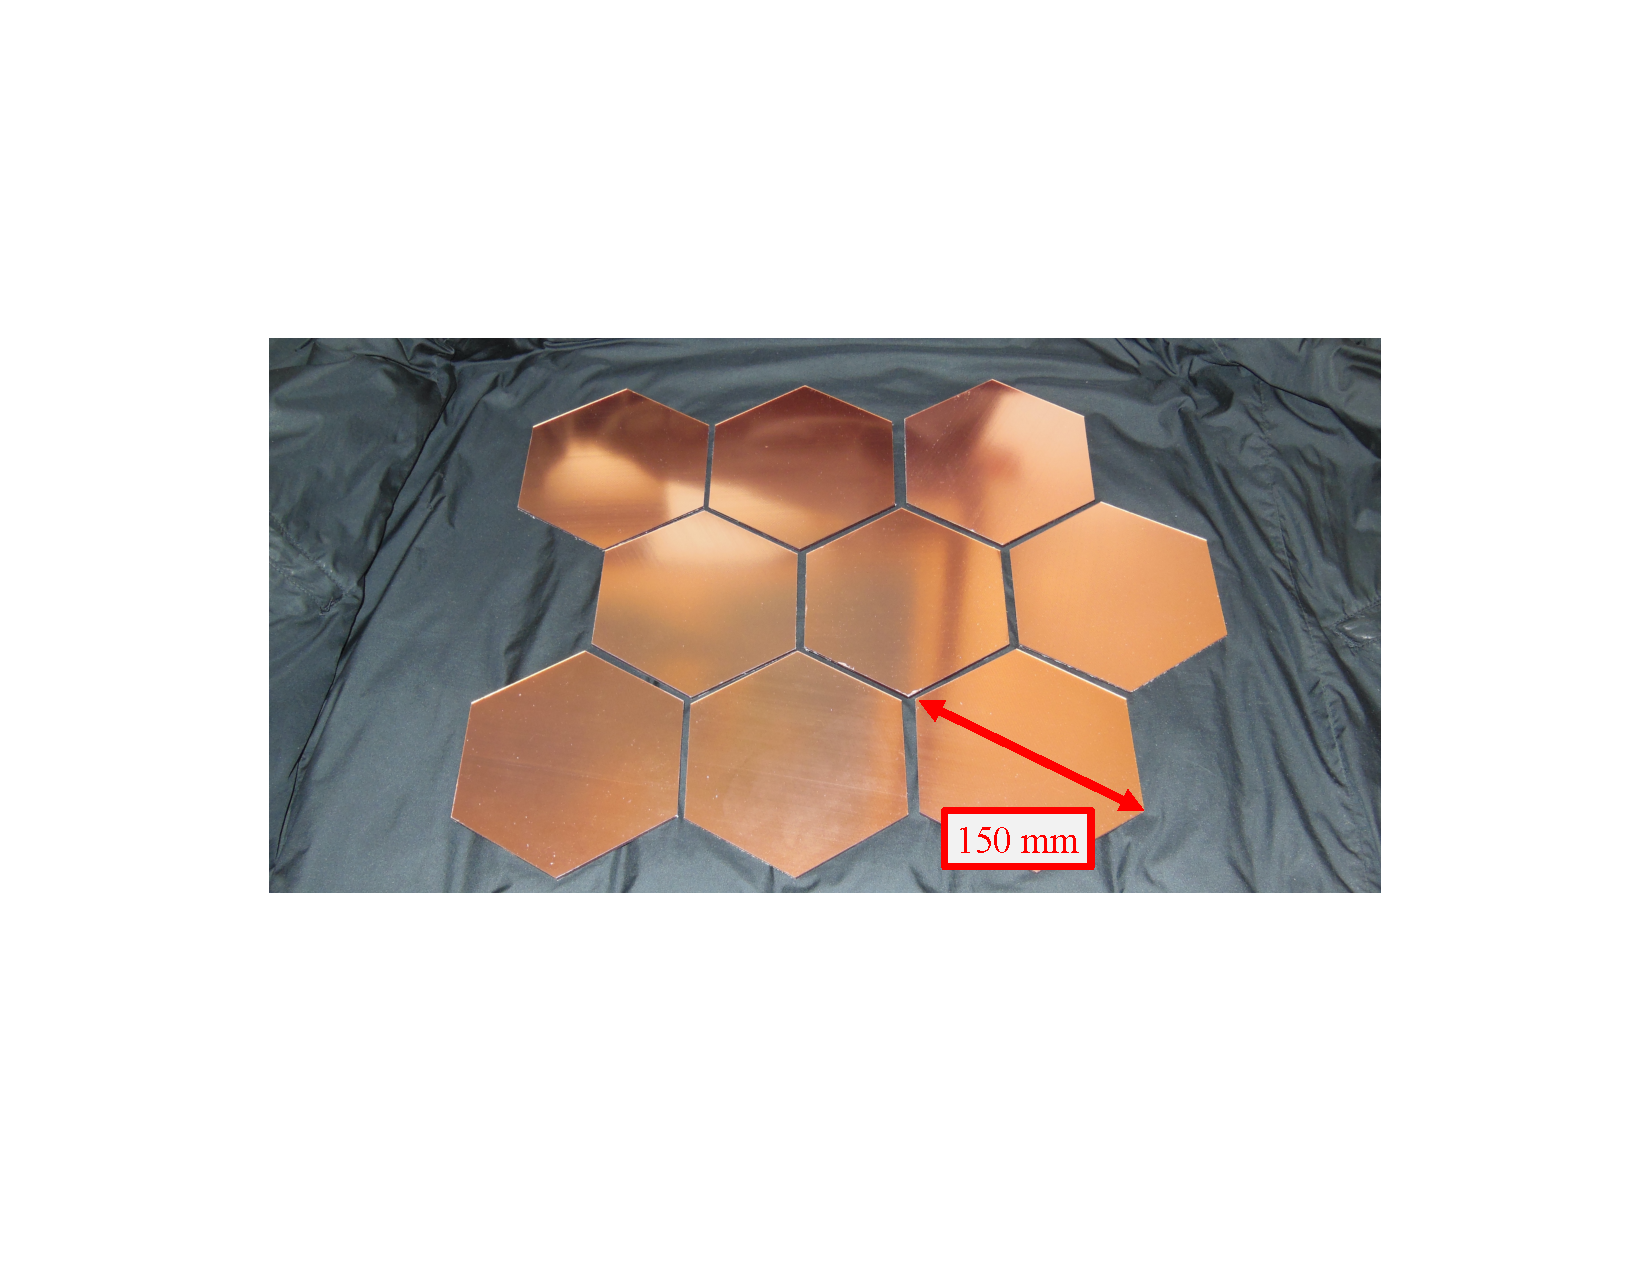
\includegraphics[width=0.48\linewidth, trim=7.2cm 5cm 7cm 5cm, clip]{InstrumentOverview/Figures/MMF_photo.pdf}}
    \caption{Caption}
    \label{fig:pb2_filters}
\end{figure}

The receiver cryostat consists of three stages, which are shown in Figure~\ref{fig:pb2_telescope}: the 50~K stage, 4~K stage, and mK stage. The 50 and 4~K stages are cooled by two Cryomech PT-415 pulse-tube refrigerators (PTRs), one of which is connected to the optics tube near the field lens, and the other of which is connected to the \important{backend} (BE). This dual-cooler system distributes the cryogenic load, dumping most of the radiative power on the OT PTR and most of the wiring-induced conductive load onto the BE PTR. Each PTR has two stages, one of which sinks $\sim$~tens of watts on the 50~K stage and another that sinks $\sim$~1~W on the 4~K stage. Given this configuration, the cryostat is built as a Russian doll of concentric shells from 300~K (the vacuum shell) to 4~K, each mounted with hollow G10 tubes, which have a low thermal conductivity, and covered with \important{multi-layer insulation} (MLI) to limit radiative loads. The mK stage is cooled by a \important{Helium-3 refrigerator}, which leverages the low boiling point of the $\mathrm{He_{3}}$ isotope to cool the focal plane to $\approx$~0.3~K. The cooling power of the mK fridge is only $\sim$~5~$\mathrm{\mu W}$, and because entropic transfer is obtained by boiling $\mathrm{He_{3}}$, the fridge must be recharged every day or two and therefore has a sub-unity duty cycle. 

In order to both keep the focal plane cold, the SA optics include a combination of absorptive and reflective IR filters. The absorptive filters are made of alumina and include a 2~mm thick flat piece at 50~K as well as the lenses at 4~K, which in addition to being refractors are good IR absorbers. These alumina optics are designed to absorb radiation $\gtrsim$~1~THz and are mounted to have high thermal conductivity to the 4~K stage, which is in turn tightly coupled to the PTC. In addition, alumina has a high thermal conductivity, which is important for keeping the optics close to isothermal and hence avoid radial thermal gradients between the optic's center (where most of the IR power propagates) and its edge (where it is thermally sunk). The reflective filters are developed at Cardiff University and are a metamaterial-layer, capacitive grid that act as low-pass reflectors.

The effectiveness of the absorptive filters relies on their conductivity to their respective cryogenic stage, and therefore much attention is payed to how the alumina optics are mounted. This strapping task is made even more challenging by the differential coefficient of thermal expansion (CTE) between the aluminum cryogenic stage and the alumina IR filter. Alumina has a CTE of $\approx$~5~ppm/C, while alumina has a CTE of $\approx$~30~ppm/C, and therefore we cannot clamp the alumina optics directly to the alumina stage without risking fracturing the alumina.

While the SO design shares many of the same principles as that of SA, there are a few key differences that ought to be highlighted. First, SO uses silicon lenses with metamaterial AR coatings. Silicon's IR absorptivity is generally lower than that of alumina and depends strongly on its resistivity, which in turn changes with temperature. Given these constraints, the SO design relies less on the lenses and more on additional filters to reject IR radiation. Second, the SO focal planes are cooled by dilution refrigerators (DRs), which operate continuously (unity duty cycle) and provide $\sim$~100~$\mathrm{\mu W}$ of cooling power at $\approx$~0.1~K. In addition, the dilution fridge has a 1~K stage with $\sim$~10~mW of cooling power, which is used to cool the LAT Lyot stop and the SAT aperture stop, as well as the lenses. Because of the DR, the SO lenses are generally cooler than those of SA, the detector operating temperatures are lower, the observation efficiency is higher, and cooling margin on the mK stage is larger.

%%%%%%%%%%%%%%%%%%%%%%%%%%%%%%%%
%%%%%%%%%%%%%%%%%%%%%%%%%%%%%%%%
%%%%%%%%%%%%%%%%%%%%%%%%%%%%%%%%

\section{Detectors}
\label{sec:simons_array_detectors}

As discussed in Section~\ref{sec:simons_array_optics}, the telescope optics couple to the detectors through an optical coupling element (either a lenslet-coupled sinuous antenna or a feed-horn-coupled OMT) via impedance-matched transmisson lines mated to on-chip bandpass filters. At this point, the filtered radiation finally reaches a \important{transition-edge sensor bolometer} (TES), which SA and SO use to detect changes in sky power. 

%%%%%%%%%%%%%%%%%%%%%%%%%%%%%%%%
%%%%%%%%%%%%%%%%%%%%%%%%%%%%%%%%

\subsection{TES operation}
\label{sec:tes_operation}

\begin{figure}[!t]
    \centering
    \subfloat[\label{fig:bolometer_operation:a}]{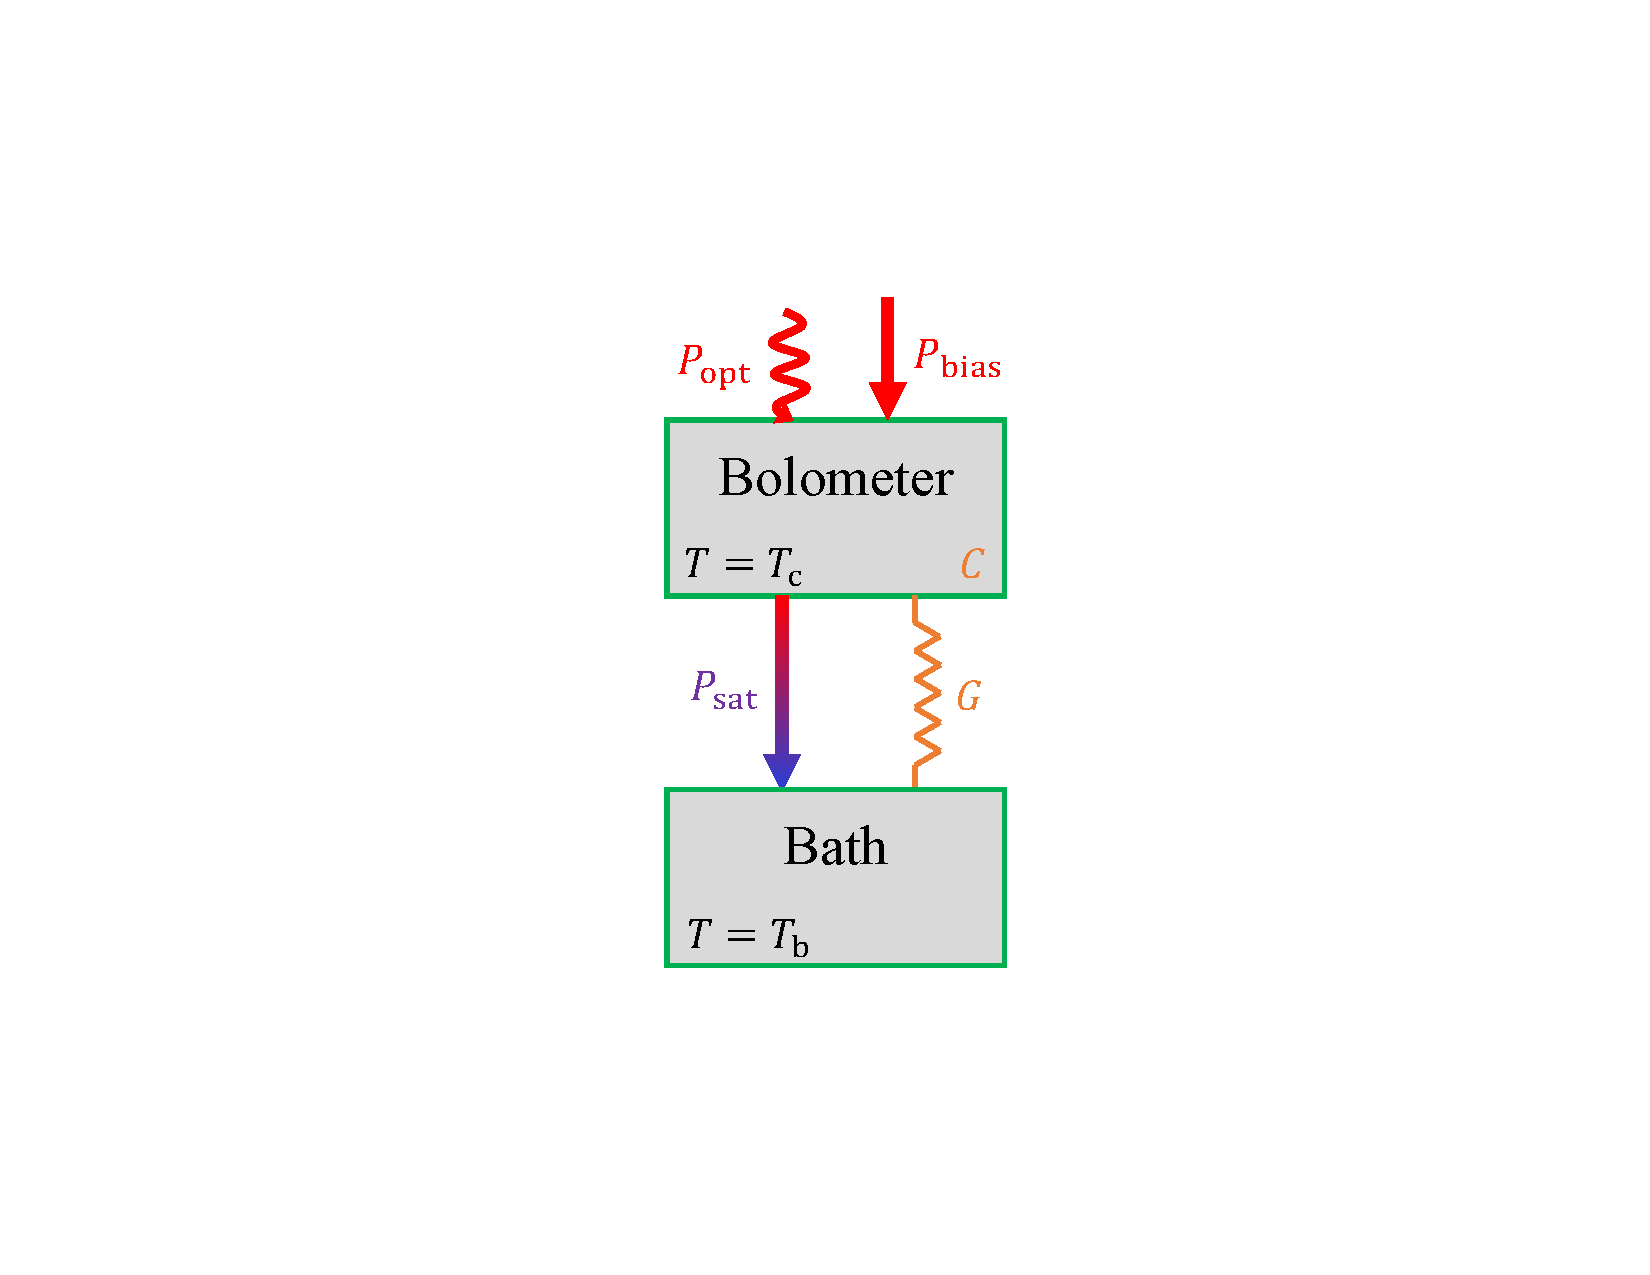
\includegraphics[width=0.35\linewidth, trim=10cm 3.5cm 10cm 5cm, clip]{InstrumentOverview/Figures/bolometer_operation.pdf}}
    \subfloat[\label{fig:bolometer_operation:b}]{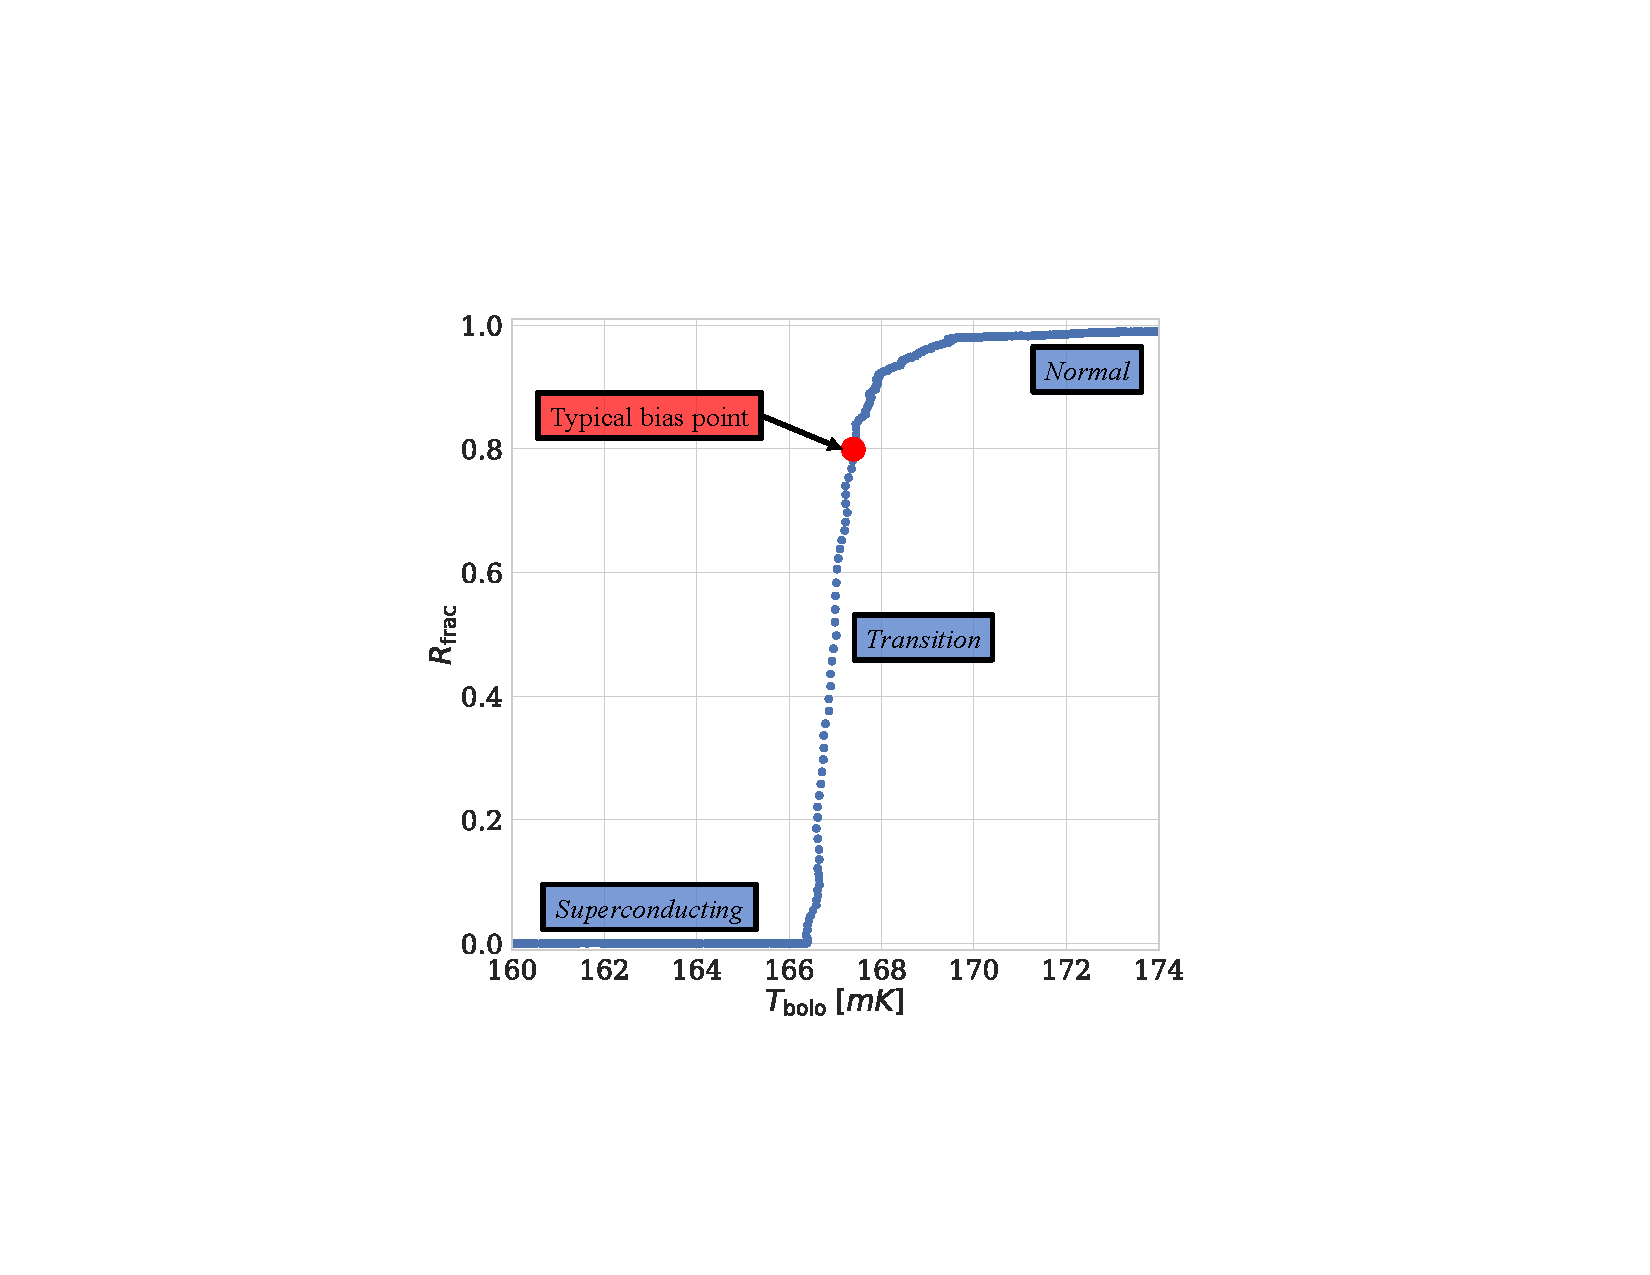
\includegraphics[width=0.63\linewidth, trim=7cm 4cm 7.5cm 5cm, clip]{InstrumentOverview/Figures/bolometer_transition.pdf}}
    \caption[Description of bolometer operation]{(a) A schematic of bolometer operation along side transition data from a TES detector for SO. The bolometer thermal element is held at its superconducting transition temperature in the presence of an optical load and an electrical (bias) load, which is balanced by a tuned thermal conduction to a thermal bath. The bias point is chosen such that, in the presence of an optical power fluctuation, $\mathrm{d}R / \mathrm{d}P_{\mathrm{opt}}$---and therefore $S = \mathrm{d}I / \mathrm{d}P_{\mathrm{opt}}$, which is called the detector responsivity---is large. In the plot on the right-hand side, the bias point is chosen to be 0.8 $\Omega$, which is approximately half of the bolometer's normal resistance.}
    \label{fig:bolometer_operation}
\end{figure}

Figure~\ref{fig:bolo_operation} shows a schematic for how the TES operates. A superconducting film is voltage biased such that the average electrical power on the bolometer is
\begin{equation}
    P_{\mathrm{bias}} = \frac{V_{\mathrm{bias}}^{2}}{R_{\mathrm{bolo}}} \, ,
    \label{eq:bolometer_p_bias}
\end{equation}
such that the total power on the bolometer is the sum of the bias power and the sky power $P_{\mathrm{opt}}$
\begin{equation}
    P_{\mathrm{tot}} = P_{\mathrm{elec}} + P_{\mathrm{opt}} \, .
    \label{eq:bolometer_power_equilibrium}
\end{equation}
The power that the TES is capable of dissipating is governed by a connection to a thermal bath with temperature $T_{\mathrm{b}}$ via a thermal link with conductivity $G$
\begin{equation}
    P_{\mathrm{sat}} = G (T_{\mathrm{c}} - T_{\mathrm{b}}) \, .
    \label{eq:saturation_power}
\end{equation}
This \important{saturation power} dictates both how much power the bolometer can absorb before saturating and how much power is due to electrical bias vs. optical power in a given optical environment. Explicitly, during normal operation, $P_{\mathrm{tot}} = P_{\mathrm{sat}}$. 

To most easily understand the bolometer's behavior in the presence of changing sky signal, consider a single Fourier mode with angular frequency $\omega$ of the optical power
\begin{equation}
    P_{\mathrm{tot}} + \delta P_{\mathrm{opt}}e^{i \omega t} + \frac{\\d P_{\mathrm{bias}}}{\\d T} \delta T e^{i \omega t} = G (T_{\mathrm{c}} - T_{\mathrm{b}}) + (g + i \omega C) \delta T e^{i \omega t} \, .
    \label{eq:changing_bolometer_power}
\end{equation}
Here, $g = \delta P / \delta T$ is the \textit{dynamic} thermal conductance and $C$ is the bolometer's heat capacity, as shown in Figure~\ref{fig:bolo_operation}. Isolating the time-varying parts gives
\begin{equation}
    \delta P_{\mathrm{opt}} = \left[ \frac{P_{\mathrm{bias}} \alpha}{T_{c}} + g + i \omega C \right] \delta T \, .
    \label{eq:time_varying_optical_power}
\end{equation}
This equation represents an optical-power-to-bolometer-temperature amplifier with a loop gain of
\begin{equation}
    \mathcal{L}(\omega) = - \frac{\delta P_{\mathrm{bias}}}{\delta P_{\mathrm{opt}}} = \frac{P_{\mathrm{bias}} \alpha}{g T_{c} (1 + i \omega \tau_0)}  = \frac{\mathcal{L}}{1 + i \omega \tau_{0}} \, .
\end{equation}
where $\mathcal{L} = P_{\mathrm{bias}} \alpha / (g T_{c})$ is the open loop gain. The bolometer's responsivity is defined to be the change in current it outputs vs change in optical power
\begin{equation}
    S_{\mathrm{I}} \equiv \frac{\dd I}{\dd P_{\mathrm{opt}}} = \frac{-\tilde{S}_{\mathrm{fact}}}{V_{\mathrm{bias}}} \frac{\mathcal{L}}{\mathcal{L} + 1} \frac{1}{1 - i \omega \tau} \, ,
    \label{eq:bolometer_responsivity}
\end{equation}
where the time constant is $\tau = (C / G) / (\mathcal{L} + 1)$ and where the responsivity factor depends on whether the bolometer is AC or DC biased
\begin{equation}
    \tilde{S}_{\mathrm{fact}} = 
    \begin{cases}
        1        & \text{if } V_{\mathrm{bias}} \mathrm{\; is \; DC} \\
        \sqrt{2} & \text{if } V_{\mathrm{bias}} \mathrm{\; is \; AC \; RMS}
    \end{cases}
    \label{eq:readout_responsivity}
\end{equation}
In the limit of high loop gain, the responsivity becomes
\begin{equation}
    S_{\mathrm{I}} \approx - \frac{\tilde{S}_{\mathrm{fact}}}{V_{\mathrm{bias}}} \;\;\; \mathrm{if} \;\;\; \mathcal{L} \gg 1 \, .
    \label{eq:responsivity_high_loop_gain}
\end{equation}

The most important characteristics of the TES bolometer are (1) when it is voltage biased, it is stabilized by \important{electrothermal feedback}, namely that $\frac{\dd P_{\mathrm{bias}}}{\dd T}$ is negative
\begin{equation}
    \frac{\dd P_{\mathrm{bias}}}{\dd T} = - \frac{V_{\mathrm{bias}}^{2}}{R^{2}} \frac{\dd R}{\dd T} \, ,
    \label{eq:electrothermal_feedback}
\end{equation}
(2) that $\frac{\dd R}{\dd T}$ is large enough to provide a large loop gain, and (3) that its impedance is low. The final point is important for how the bolometer current signal is amplified, which we discuss below.

%%%%%%%%%%%%%%%%%%%%%%%%%%%%%%%%
%%%%%%%%%%%%%%%%%%%%%%%%%%%%%%%%

\subsection{TES readout}
\label{sec:tes_readout}

In order to digitize the detector signals, both SA and SO multiplex TES readout using superconducting quantum interference devices (SQUIDs). SQUIDs are transimpedance amplifiers with low input impedance and large gain, and they operate by sensing current changes across the bolometer (as in Equation~\ref{eq:bolometer_responsivity}) using Josephson junctions. SQUIDs are suitable to read $\mu A$ currents across a large bandwidth ($\sim$~100~GHz), and their low input impedance makes them well-suited for TESes, which operate at low resistances ($\sim$~1~$\Omega$ for SA, $\sim$~10~$m \Omega$ for SO). Multiplexed readout enables many mK detectors to be sensed on one 4~K amplifier, decreasing the number of wires that need to run from the 4~K stage to the mK stage, in turn reducing the thermal load on the focal plane. SA uses a technique called \important{digital frequency multiplexing} (dfMUX), while SO uses a technique called \important{microwave multiplexing} ($\mathrm{\mu}$MUX), both of which we briefly overview below.

\begin{figure}[!t]
    \centering
    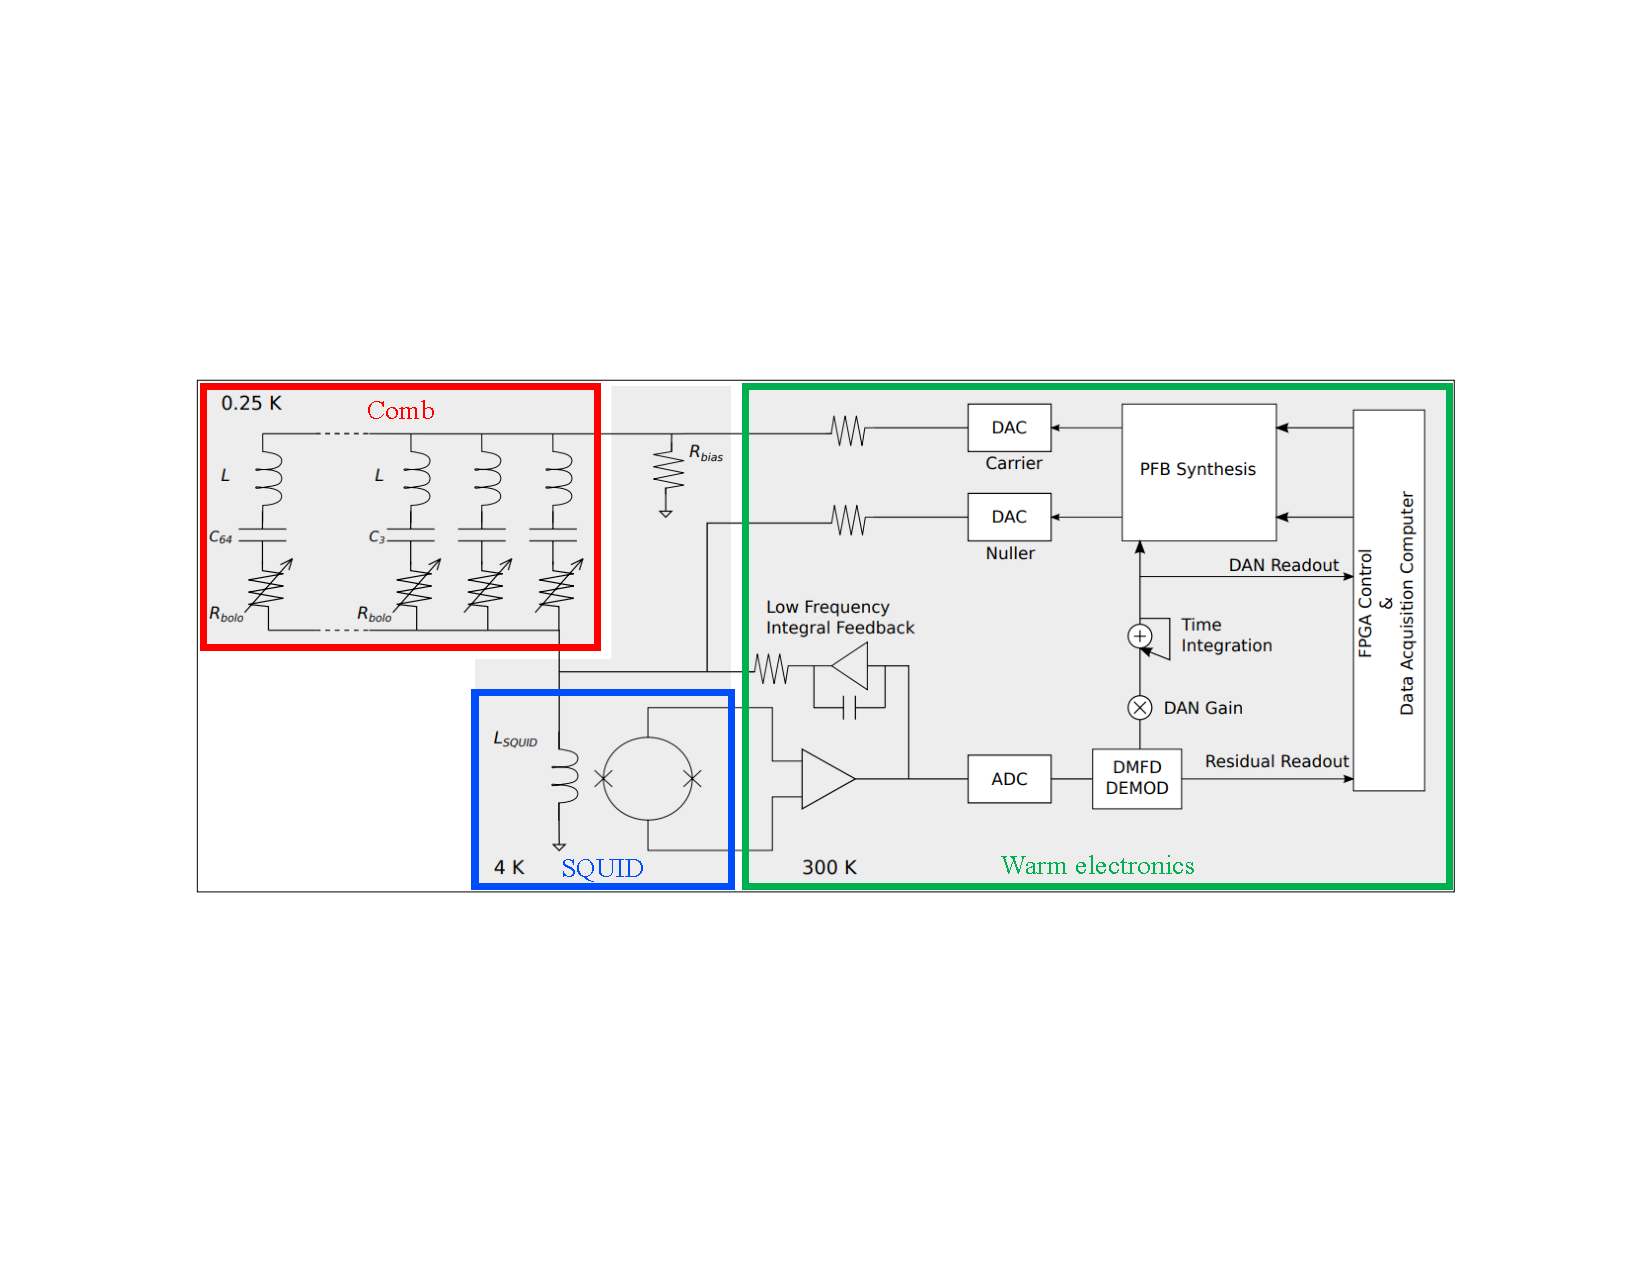
\includegraphics[width=\linewidth, trim=3cm 6.3cm 3cm 6.3cm, clip]{InstrumentOverview/Figures/dfmux_readout.pdf}
    \caption{Caption}
    \label{fig:dfmux_readout}
\end{figure}

SA's dfMUX scheme reads out 38 mK bolometers per 4~K SQUID at MHz frequencies. Each bolometer's bias/readout frequency is constructed by placing it in series with a tuned \important{LC resonator}, creating a ``comb'' of 38 low-impedance, non-overlapping ``peaks'' between 1~$\sim$~5~MHz. These frequency channels are then biased by a matching comb of AC waveforms, and when sky power changes on a given channel, this results in a change in the AC current across the bolometer. All 38 current waveforms are fed to one SQUID, are amplified into voltages, and are further amplified subsequently demodulated by a system of ambient electronics.

\begin{figure}[!t]
    \centering
    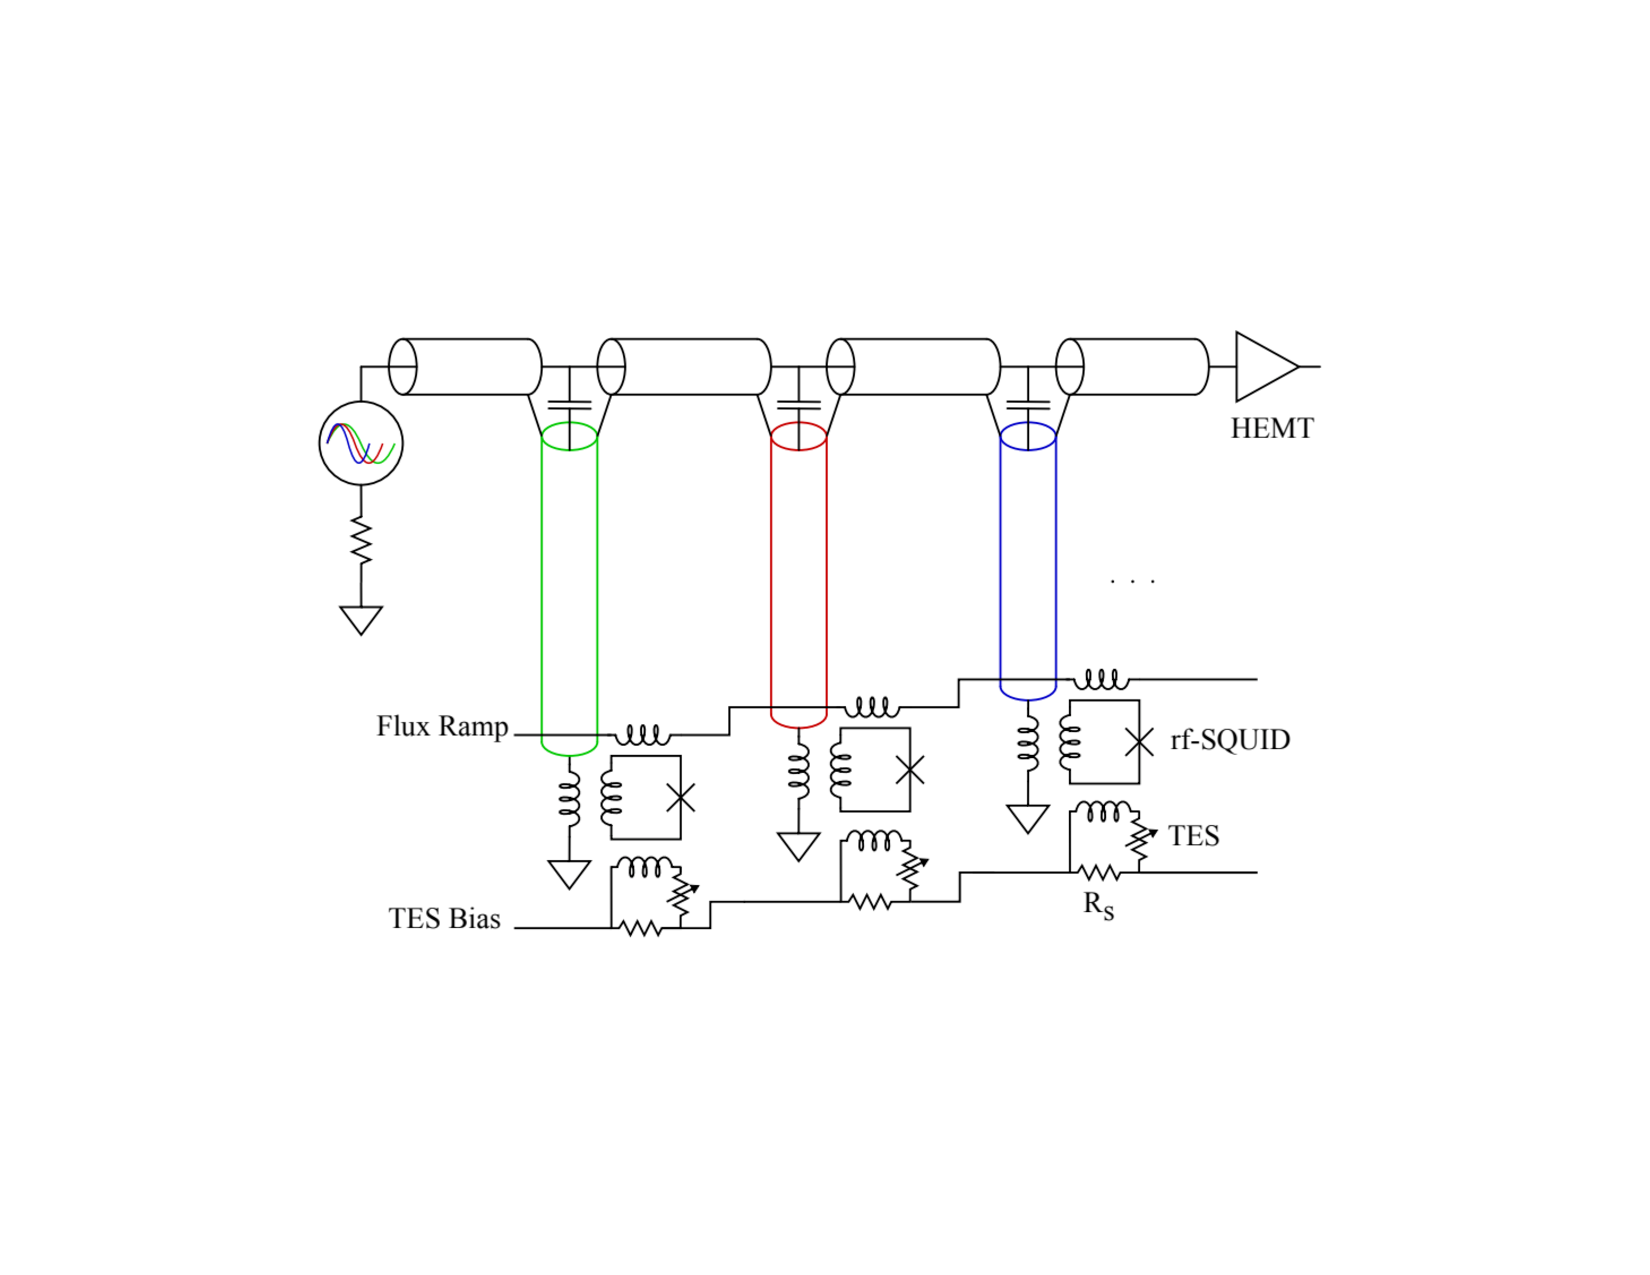
\includegraphics[width=\linewidth, trim=4cm 5.5cm 4cm 5cm, clip]{InstrumentOverview/Figures/umux_readout.pdf}
    \caption{Caption}
    \label{fig:umux_readout}
\end{figure}

SO's $\mathrm{\mu}$MUX scheme reads out $\sim$~1,000 mK bolometers coupled to $\sim$~1,000 mK SQUIDs (one SQUID per bolometer) per 4~K high-electron-mobility transistor (HEMT) amplifier at GHz frequencies. Instead of putting an LC resonator in series with the bolometer and using the same tone to both bias bolometer and sense its resistance changes, SO decouples the signal used to read out the bolometer and the signal used to bias it. As shown in Figure~blah, the TESes are biased with a DC voltage and are in series with an inductor. This inductor is coupled to a SQUID, which is in turn inductively coupled to an LC resonator. When the current across the bolometer changes, so does the SQUID-resonator effective inductance, in turn modulating the LC resonant frequency. When the resontator's impedance changes, so does the reflected signal, which is amplified by a broadband high-electron-mobility transistor (HEMT) amplifier and subsequently digitized by warm electronics. Because the probe (the LC resonator biases) and the bolometer voltage bias are separate in this scheme, $\mathrm{\mu}$MUX can operate at much higher frequencies and therefore multiplex more detectors on each amplifier.

While dfMUX and $\mathrm{\mu}$MUX are powerful techniques to read out the bolometer array, they have many challenges two of which are important for discussion to follow. First is bolometer responsivity, which is governed by its loop gain and depends heavily on implementation details, including the high-frequency impedances of the wiring, the effectiveness of the electromagnetic shielding, and the uniformity and consistency of the detector and resonator fabrication. Parasitic effects at high frequencies can be difficult to control and therefore can lead to substantial variations in how sky power is converted to analog-to-digital converter (ADC) counts. Second is readout noise, which depends on a plethora of factors, including SQUID noise, grounding quality, and detector bias parameters. Many of these factors are particularly prominent at higher frequencies and therefore are critical for dfMUX and $\mathrm{\mu}$MUX as opposed to other readout schemes (such as time-domain multiplexing). Because SA and SO push to very low thermal and optical noise, readout noise characterization and modeling are essential to an accurate assessment of instrument sensitivity.

%%%%%%%%%%%%%%%%%%%%%%%%%%%%%%%%
%%%%%%%%%%%%%%%%%%%%%%%%%%%%%%%%

\section{Technical objectives}
